\documentclass[bj]{imsart}
\makeatletter
\def\set@curr@file#1{%
  \begingroup
    \escapechar\m@ne
    \xdef\@curr@file{\expandafter\string\csname #1\endcsname}%
  \endgroup
}
\def\quote@name#1{"\quote@@name#1\@gobble""}
\def\quote@@name#1"{#1\quote@@name}
\def\unquote@name#1{\quote@@name#1\@gobble"}
\makeatother
\usepackage{graphics}


\usepackage{lineno,hyperref}
\usepackage{amsfonts,amssymb}
\usepackage{mathtools}
%\usepackage{mathbbol}
\usepackage{bbm}
\usepackage{multirow,algorithm2e}%
\usepackage{xargs}
%\usepackage{showlabels}

\def\P{\mathsf{P}}
\def\PE{\mathsf{E}}
\def\PVar{\mathsf{Var}}
\def\PCov{\mathsf{cov}}
\newcommandx{\CPE}[3][1=]{{\mathsf E}_{#1}\left[\left. #2 \, \right| #3 \right]}
\newcommand{\ps}[2]{\langle #1, #2 \rangle}
\def\nset{\mathbb{N}}
\def\rset{\mathbb{R}}
\usepackage[textsize=footnotesize]{todonotes} % pour voir les commentaires

\newcommand{\eric}[1]{\todo[color=purple!10, author=Eric]{#1}}
\newcommand{\erici}[1]{\todo[inline,color=purple!10, author=Eric]{#1}}
\newcommand{\denis}[1]{\todo[color=green!10, author=Denis]{#1}}
\newcommand{\denisi}[1]{\todo[inline,color=green!10, author=Denis]{#1}}
\newcommand{\sergey}[1]{\todo[color=blue!10, author=Sergey]{#1}}
\newcommand{\sergeyi}[1]{\todo[inline,color=red!10, author=Sergey]{#1}}

\def\rmd{\mathrm{d}}
\def\rme{\mathrm{e}}
\def\rset{\mathbb{R}}
\def\NtrainPath{T}
\def\TrainSet{\mathcal{D}}
\modulolinenumbers[5]
\newcommand{\proofendsign}{$\Box$}
\newtheorem{thm}{Theorem}
\newtheorem{definition}{Definition}
\newtheorem{lem}[thm]{Lemma}
\newtheorem{prop}[thm]{Proposition}
\newtheorem{remark}[thm]{Remark}
\newtheorem{cor}[thm]{Corollary}
\newtheorem{example}[thm]{Example}
\newenvironment{proof}{{\noindent \bf Proof }}
 {{\hspace*{\fill}\proofendsign\par\bigskip}}
\def\TV{\operatorname{TV}}
\newcommand{\jac}[1]{\operatorname{J} _{#1}}

%added command for indicator - SS
\newcommand{\indi}[1]{\mathbbm{1}_{#1}}
\newcommand{\indiacc}[1]{\mathbbm{1}_{\{#1\}}}

\newcommand*{\argmin}{\operatornamewithlimits{arg\,min}}
\newcommand*{\const}{\mathrm{const}}
\usepackage[lofdepth,lotdepth]{subfig}
\usepackage{graphicx}
\newcommand*{\ol}{\overline}

\newcommand{\tcr}[1]{\textcolor{red}{#1}}
\newcommand{\tvnorm}[1]{\| #1 \|_{\operatorname{TV}}}
\def\kerULA{\operatorname{Q}}
\def\eqsp{\,}
\begin{document}

\begin{frontmatter}
\title{Variance reduction for Markov chains via martingale representations}
\runtitle{Variance reduction for Markov chains}
%\thankstext{T1}{This research was }


\begin{aug}
\author{\snm{D. Belomestny}\thanksref{a,b}\ead[label=e1]{denis.belomestny@uni-due.de}}
\and
\author{\snm{E. Moulines}\thanksref{c, b}\ead[label=e2]{eric.moulines@polytechnique.edu}}
\and
\author{\snm{S. Samsonov}\thanksref{b}\ead[label=e3]{svsamsonov@hse.ru}}
%\and
%\author{\snm{N. Shagadatov}\thanksref{b}\ead[label=e4]{nshagadatov@edu.hse.ru}}



\runauthor{D. Belomestny et al}

\affiliation{Duisburg-Essen University, National Research University Higher School of Economics,  Ecole Polytechnique  and Duisburg-Essen University}

\address[a]{
Duisburg-Essen University,
Faculty of Mathematics,
D-45127 Essen
Germany }

\address[c]{
Centre de Math\'ematiques Appliqu\'ees, UMR 7641, Ecole Polytechnique,
France
}

\address[b]{
National University Higher School of Economics, Moscow, Russia
}

\end{aug}

\begin{abstract}
In this paper we propose an efficient variance reduction approach for  additive functionals of Markov chains relying on a novel discrete time martingale representation. Our approach is fully non-asymptotic and does not require the knowledge of the stationary distribution (and even any type of ergodicity) or specific structure of the underlying density.  By rigorously analyzing the  convergence properties of the proposed algorithm, we show that its complexity is indeed asymptotically smaller than one of the naive algorithm. The numerical performance of the new method is illustrated for Markov Chain Monte Carlo (MCMC) methods.
\end{abstract}

\begin{keyword}[class=MSC]
\kwd[Primary ]{60G40}
\kwd{60G40}
\kwd[; secondary ]{91G80}
\end{keyword}

\begin{keyword}
\kwd{MCMC}
\kwd{variance reduction}
\kwd{martingale representation}
\end{keyword}

\end{frontmatter}

\section{Introduction}
Markov chains and Markov Chain Monte Carlo algorithms play crucial role in modern numerical analysis, finding various applications in such research areas as Bayesian inference, reinforcement learning, online learning. As an illustration, suppose that we aim at computing $\pi(f):= \PE\left[f(X)\right]$, where $X$ is a random vector in $\mathcal{X} \subseteq \rset^d$ admitting a density $\pi$ and $f$ is a square-integrable function $f:\mathcal{X} \to \rset$, $f \in L^2(\pi)$. Typically it is not possible to compute $\pi(f)$ analytically, leading to the Monte Carlo methods as a popular solution. Given an independent identically distributed observations $X_1,\ldots,X_n$ from $\pi$, we might estimate $\pi(f)$ by $\hat{\pi}(f):=1/n\sum_{k=1}^{n}f(X_k)$. The variance of such estimate equals $\sigma^2(f)/n$  with $\sigma^2(f)$ being the variance of the integrand. The first way to obtain tighter estimate $\hat{\pi}(f)$ is simply to increase the sample size $n$. Unfortunately, this solution might be prohibitively costly, especially when the dimension $d$ is large enough or sampling from $\pi$ is complicated. An alternative approach is to decrease $\sigma^2(f)$ by constructing a new Monte-Carlo experiment with the same expectation as the original one, but with a lower variance. Methods to achieve this are known as variance
reduction techniques. Introduction to many of them can be found in \cite{rubinstein2016simulation}, \cite{GobetBook} and \cite{glasserman2013monte}. Recently one witnessed a revival of interest in efficient variance reduction methods  for Markov chains, mostly with applications to MCMC algorithms; see for example \cite{dellaportas2012control}, \cite{mira2013zero}, \cite{oates:girolami:chopin:2016}, \cite{south:mira:drovandi:2018}, \cite{brosse2018diffusion} and references therein.
\par
One of the popular approaches to variance reduction is the control variates method. We aim at constructing cheaply computable random variable $\zeta$ (control variate) with $\PE[\zeta] = 0$ and $\PE[\zeta^2] < \infty$, such that the variance of the r.v. $f(X) + \zeta$ is small. The complexity of the problem of constructing classes $Z$ of control variates \(\zeta\) satisfying   $\PE[\zeta]=0$ essentially depends on the degree of our knowledge on \(\pi.\)
For example, if \(\pi\) is analytically known and satisfies some regularity conditions, one can apply the well-known technique of  polynomial interpolation to construct control variates enjoying  some optimality properties, see, for example \cite[Section~3.2]{dimov2008monte}. Alternatively, if an orthonormal system in \(L^2(\pi)\) is analytically available, one can build control variates \(\zeta\) as a linear combination of the corresponding basis functions, see \cite{GobetCV}. Furthermore, if \(\pi\) is known only up to a normalizing constant (which is often the case in Bayesian statistics), one can apply the recent approach of control variates  depending only on the gradient \(\nabla \log \pi\)  using Schr\(\ddot{\text{o}}\)dinger-type Hamiltonian operator in  \cite{assaraf1999zero}, \cite{mira2013zero}, and Stein operator in \cite{brosse2018diffusion}.
In some situations \(\pi\) is not known analytically, but \(X\) can be represented as a function of  simple random variables with known distribution.
Such  situation arises, for example, in the case of functionals of  discretized diffusion processes. In this case a Wiener chaos-type decomposition can be used to construct control variates with nice theoretical properties, see \cite{belomestny2018stratified}.
Note that in order to compare different  variance reduction approaches, one has to analyze their complexity, that is, the number of numerical operations required to achieve a prescribed magnitude of the resulting variance.
\par
Unfortunately it is not always possible to generate independent observations distributed according to $\pi$. To overcome this issue one might consider MCMC algorithms, where the exact samples from $\pi$ are replaced by \((X_p),\) \(p=0,1,2,\ldots,\) forming a Markov chain with a marginal distribution of $X_n$ converging to $\pi$ in a suitable metrics as $n$ grows. It is still possible to apply the control variates method in the similar manner to a simple Monte-Carlo case, yet the choice of the optimal control variate becomes much more difficult. Due to significant correlations between the elements of the Markov chain it might be not enough to minimize the marginal variances of \((X_p)_{p \geq 0}\) as it was in independent case. Instead one may choose the control variate by minimizing the corresponding asymptotic variance of the chain as it is suggested in~\cite{belomestny2019esvm}. At the same time it is possible to express the optimal control variate in terms of the solution of the Poisson equation for the corresponding Markov chain \((X_p)\). As it was observed in~\cite{henderson1997variance,henderson2004}, for a time-homogeneous Markov chain \(X_p\) with a stationary distribution \(\pi\), the function $U_{G}(x) := G(x)-\PE[G(X_{1})|X_0 = x]$ has a zero mean with respect to $\pi$ for arbitrary real-valued function \(G: \mathcal{X} \to \rset\), such that \(G  \in L^1(\pi)\). Hence, $U_{G}(x)$ is a valid control functional for a suitable choice of $G$, with the best $G$ given by a solution of the Poisson equation \(\PE [G(X_{1})|X_0 = x]-G(x)=-f(x)+\pi(f)\). For such $G$ we obtain $f(x) + U_G(x) = f(x) - f(x) + \pi(f) = \pi(f)$ leading to an ideal estimator with zero variance. Despite the fact that the Poisson equation involves the quantity of interest \(\pi(f)\)  and can not be  solved explicitly in most cases, this idea still can be used to construct some  approximations for the optimal zero-variance control variates. For example,  \cite{henderson1997variance} proposed to compute approximations for the solution of the Poisson equation for specific Markov chains with particular emphasis on models arising in stochastic network theory. In \cite{dellaportas2012control} and \cite{brosse2018diffusion}  series-type control variates are introduced and studied for reversible Markov chains. It is assumed in \cite{dellaportas2012control}  that the one-step conditional expectations  can be computed explicitly  for a set of basis functions. The authors in \cite{brosse2018diffusion} proposed another approach tailored to diffusion setting which does not require the computation of integrals of basis functions and only involves  applications of the underlying generator.
\par
In this paper we focus on the  Langevin type algorithms which got much attention recently, see \cite{dalalyan2017theoretical,durmus:moulines:2017, MR2353037, MR3861816, MR2977986} and references therein. We propose  a generic variance reduction method for these and other types algorithms, which is purely non-asymptotic and does not require that    the conditional expectations of the corresponding Markov chain can be computed  or that the generator is known analytically. Moreover, we do not need to assume stationarity or/and sampling under the invariant distribution \(\pi.\) We rigorously analyse the convergence of the method and study its complexity. It is shown that  our variance-reduced Langevin algorithm outperforms the standard Langevin algorithms in terms of complexity.
\par
The paper is organized as follows.  In Section~\ref{sec:setup} we set up the problem and introduce some notations. Section~\ref{seq:mart_repr} contains a novel martingale representation and shows how this representation can be used for variance reduction. In Section~\ref{sec:ula_analysis} we analyze the performance of the proposed variance reduction algorithm in the case of Unadjusted Langevin Algorithm (ULA).  Finally, numerical examples are presented in Section~\ref{sec:num}.

\paragraph{Notations. }\label{par:notations}
We use the notations $\nset=\{1,2,\ldots\}$ and $\nset_0=\mathbb N\cup\{0\}$. We denote $\boldsymbol{\varphi}(z)=(2\pi)^{-d/2} \exp(-|z|^2/2)$, $z\in\mathbb R^d$ probability density function of the $d-$dimensional standard normal distribution. For $x \in \rset^d$ and $r>0$ let $B_r(x) = \{y \in \rset^d | \|y - x\| < r\}$ where $\|\cdot\|$ is a standard Euclidean norm. For the twice differentiable function $g: \rset^d \rightarrow \rset$ we denote by $D^2g(x)$ its Hessian at point $x$. For $m\in\mathbb N$, a smooth function
$h\colon\mathbb R^{d\times m}\to\mathbb R$
with arguments being denoted
$(y_1,\ldots,y_m)$, $y_i\in\mathbb R^d$, $i=1,\ldots,m$,
a multi-index $\mathbf k=(k_i)\in\mathbb N_0^d$,
and $j\in\{1,\ldots,m\}$,
we use the notation $\partial^{\mathbf k}_{y_j} h$ for the multiple derivative of $h$
with respect to the components of~$y_j$:
\[
\partial^{\mathbf k}_{y_j} h(y_1,\ldots,y_m)
:=\partial^{k_d}_{y_j^d}
\ldots
\partial^{k_1}_{y_j^1}
h(y_1,\ldots,y_m),
\quad y_j=(y_j^1,\ldots,y_j^d).
\]
In the particular case $m=1$ we drop the subscript $y_1$ in that notation. For probability measures $\mu$ and $\nu$ on $\rset^d$ denote by $\tvnorm{\mu-\nu}$ the total variation distance between $\mu$ and $\nu$, that is,
\[
\tvnorm{\mu-\nu}=\sup_{A \in \mathcal{B}(\rset^d)}
|\mu(A)-\nu(A)| \eqsp.
\]
where $\mathcal{B}(\rset^d)$ is a Borel $\sigma$-algebra of $\rset^d$. For a bounded Borel function $f: \rset^d \rightarrow \rset$ denote $\mathrm{osc}(f):=\sup_{x\in\mathbb R^d}f(x)-\inf_{x\in\mathbb R^d}f(x)$. Given a function $V: \rset^d \rightarrow \rset$, for a function $f: \rset^d \rightarrow \rset$ we define $\|f\|_{V} = \sup_{x \in \rset^d} |f(x)|/V(x)$ and the corresponding $V-$norm between probability measures $\mu$ and $\nu$ on $\mathcal{B}(\rset^d)$ as
\[
d_V(\mu, \nu) = \|\mu - \nu\|_{V} = \sup_{\|f\|_{V} \leq 1} \left[\int\nolimits_{\rset^d}f(x)\,d\mu(x) - \int\nolimits_{\rset^d}f(x)\,d\nu(x)\right]  \eqsp.
\]


\section{Setup}\label{sec:setup}
Let  \(\mathcal{X}\) be a domain in \( \mathbb{R}^d.\)  Our aim is to numerically compute  expectations of the form
\[
\pi(f)=\int_{\mathcal{X}} f(x)\pi(\rmd x),
\]
where \(f:\) \(\mathcal{X}\longrightarrow \mathbb{R}\) and \(\pi\) is a probability measure supported on \(\mathcal{X}.\)
If  the dimension of the space \(\mathcal{X}\) is large and \(\pi(f)\) can not be computed analytically, one can apply Monte Carlo methods. However, in many practical situations  direct sampling from \(\pi\) is impossible and this precludes the use of plain Monte Carlo methods in this case. One popular alternative to Monte Carlo  is Markov Chain Monte Carlo (MCMC), where one is looking for a discrete time  (possibly non-homogeneous) Markov chain   \((X_p)_{p \in \nset_0}\) such that \(\pi\) is its unique invariant measure. In this paper we study a class of MCMC algorithms with \((X_p)_{p \in \nset_0}\) satisfying the  the following recurrence relation:
\begin{equation}
\label{eq:chain_gen}
X_{p}=\Phi_{p}(X_{p-1},\xi_{p}),\quad p=1,2,\ldots ,\quad X_{0}=x,
\end{equation}
for some i.i.d.  random vectors \(\xi_p\in \mathbb{R}^m\) with distribution \(P_{\xi}\)
and some Borel-measurable
functions $\Phi_{p}\colon\mathcal{X}\times\mathbb{R}^{m}\to\mathcal{X}.$
In fact, this is quite general class of Markov chains (see \cite[Theorem~1.3.6]{moulines2018})
and many well-known MCMC algorithms can be represented in the form \eqref{eq:chain_gen}.
Let us consider two popular examples.
\begin{example}[Unadjusted Langevin Algorithm]
\label{exam:langevin-algorithm}
Fix a sequence of positive time steps \((\gamma_p)_{p\geq 1}.\) Given a Borel function $\mu\colon\mathbb{R}^{d}\to\mathbb{R}^{d}$,
consider a non-homogeneous
discrete-time Markov chain $(X_{p})_{p\geq0}$ defined by
\begin{equation}\label{eq:chain}
X_{p+1}=X_{p}-\gamma_{p+1}\mu(X_{p})+\sqrt{\gamma_{p+1}}Z_{p+1},\end{equation}
where $\left(Z_{p}\right)_{p\geq1}$ is an i.i.d.\ sequence of $d$-dimensional
standard Gaussian random vectors. If
$\mu= \nabla U$
for some continuously differentiable function $U,$ then Markov chain~\eqref{eq:chain} can be used to approximately sample from the density
\begin{equation}\label{eq:stationary_distr}
\pi(x)= Z^{-1} \rme^{-U(x)/2}, \quad Z= \int_{\mathbb{R}^{d}} \rme^{-U(x)/2}\, \rmd x,
\end{equation}
provided that \(Z < \infty\).
This method is usually referred to as Unadjusted Langevin Algorithm (ULA).
Denote by \(W\) the standard \(\mathbb{R}^m\)-valued Brownian motion.
The Markov chain~\eqref{eq:chain}
arises as the Euler-Maruyama discretization
of the Langevin diffusion
\[
\rmd Y_t=-\mu(Y_t)\,\rmd t+ \rmd W_t
\]
with nonnegative time steps $(\gamma_p)_{p\ge1}$,
and,  under mild technical conditions, the latter Langevin diffusion admits $\pi$
of~\eqref{eq:stationary_distr}
as its unique invariant distribution; see \cite{dalalyan2017theoretical} and \cite{durmus:moulines:2017}.
\end{example}
\begin{example}[Metropolis-Adjusted Langevin Algorithm]
The Metropolis-Hastings algorithm
associated with a target density \(\pi\) requires the choice of a sequence of conditional densities  \((q_p)_{p\geq 1}\) also called proposal or candidate kernels. The transition from the value  of the Markov chain \(X_p\)  at time \(p\)
and its value at time \(p + 1\) proceeds via the following transition step:

\begin{algorithm}[H]
Given \(X_p=x\)\;
\begin{enumerate}
\item Generate \(Y_p\sim q_p(\cdot|x)\)\;
\item Put
\begin{eqnarray*}
X_{p+1}=
\begin{cases}
Y_p, & \texttt{ with probability } \alpha_p(x,Y_p),
\\
x, &  \texttt{ with probability } 1-\alpha_p(x,Y_p),
\end{cases}
\end{eqnarray*}
where
\begin{eqnarray*}
\alpha_p(x,y)=\min\left\{1,\frac{\pi(y)}{\pi(x)}\frac{q_p(x|y)}{q_p(y|x)}\right\}.
\end{eqnarray*}
\end{enumerate}
\end{algorithm}
This transition is reversible with respect to \(\pi\) and therefore preserves the stationary density \(\pi\); see \cite[Chapter~2]{moulines2018}. If \(q_p\) have a wide enough
support to eventually reach any region
of the state space \(\mathcal{X}\) with positive mass
under \(\pi\), then this transition is irreducible and $\pi$ is a maximal irreducibility measure \cite{mengersen:tweedie:1996}. The  Metropolis-Adjusted Langevin algorithm (MALA) takes  \eqref{eq:chain} as proposal, that is,
\begin{eqnarray*}
q_p(y|x)=(\gamma_{p+1})^{-d/2}\boldsymbol{\varphi}\Bigl([y-x+\gamma_{p+1}\mu(x)]/\sqrt{\gamma_{p+1}}\Bigr) \,.
\end{eqnarray*}
The MALA algorithms usually provide noticeable speed-ups in convergence for most problems. It is not difficult to see that the MALA chain can be compactly represented in the form
\begin{align*}
X_{p+1} &=X_p+\mathbbm{1}\bigl(U_{p+1}\leq \alpha(X_{p},Y_{p})\bigr)(Y_{p}-X_p),  \,
Y_{p}&=X_p-\gamma_{p+1}\mu(X_p)+\sqrt{\gamma_{p+1}}Z_{p+1},
\end{align*}
where \((U_{p})_{p\geq 1}\) is an i.i.d. sequence of uniformly distributed on \([0,1]\) random variables independent of \((Z_p)_{p\geq 1}.\) Thus we recover \eqref{eq:chain_gen} with  \(\xi_p=(U_p,Z_p)\in \mathbb{R}^{d+1}\) and
\begin{eqnarray*}
\Phi_p(x,(u,z)^\top)=x+\mathbbm{1}\bigl(u\leq \alpha(x,x-\gamma_{p}\mu(x)+\sqrt{\gamma_{p}}z)\bigr)(-\gamma_{p}\mu(x)+\sqrt{\gamma_{p}}z).
\end{eqnarray*}
\end{example}
\begin{example}
  Let \((X_t)_{t\in [0,T]}\) be the unique strong solution to a  SDE of the form:
\begin{eqnarray}
\label{eq:sde-inv}
\rmd X_t=b(X_t)\, \rmd t+\sigma(X_t)\, \rmd W_t,\quad t\geq 0,	
\end{eqnarray}
where \(b:\) \(\mathbb{R}^d\to \mathbb{R}^d\) and \(\sigma:\) \(\mathbb{R}^d\times \mathbb{R}^m \to \mathbb{R}^d\) are locally Lipschitz continuous functions with at most linear growth.
The process \((X_t)_{t\geq 0}\) is a Markov
process and let \(L\) denote its infinitesimal generator defined by
\begin{equation*}
Lg=b^\top \nabla g+\frac{1}{2}\sigma^\top D^2g\sigma
\end{equation*}
for any \(g\in C^2(\mathbb{R}^d).\)
If there exists a continuously twice differentiable Lyapunov function \(V:\) \(\mathbb{R}^d\to \mathbb{R}_{+}\) such that
\begin{eqnarray*}
\sup_{x\in \mathbb{R}^d} LV(x) <\infty,\quad \limsup_{|x|\to \infty} LV(x)<0,
\end{eqnarray*}
then there is an invariant probability measure \(\pi\)  for \(X,\) that is, \(X_t\sim \pi\) for all \(t> 0\) if \(X_0\sim \pi.\) Invariant measures are crucial in the study of the long term behaviour of stochastic differential
systems \eqref{eq:sde-inv}.    Under some additional assumptions,  the invariant
measure \(\pi\) is  ergodic and this property
can be exploited  to compute  the integrals \(\pi(f)\) for \(f\in L^2(\pi)\) by means of ergodic averages. The idea is to replace the diffusion \(X\) by a (simulable) discretization scheme of the form (see e.g. \cite{MR3861816})
\begin{eqnarray*}
\bar X_{n+1}=\bar X_n+\gamma_{n+1} b(\bar X_n)+\sigma(\bar X_n)(W_{\Gamma_{n+1}}-W_{\Gamma_n}), \quad n\geq 0,\quad \bar X_0=X_0,
\end{eqnarray*}
where \(\Gamma_n=\gamma_1+\ldots+\gamma_n\) and \((\gamma_n)_{n\geq 1}\) is a non-increasing sequence of time steps. Then for a function \(f\in L^2(\pi)\) we can approximate \(\pi(f)\) via
\begin{eqnarray*}
\pi_n^\gamma(f)=\frac{1}{\Gamma_n}\sum_{i=1}^n \gamma_{i}f(\bar X_{i-1}).
\end{eqnarray*}
Due to typically high correlation between \(X_0,X_1,\ldots\)  variance reduction is of crucial importance here.
As a matter of fact, in many cases there is no explicit formula for the invariant measure and this makes the use of gradient  based  variance reduction techniques (see e.g. \cite{mira2013zero}) impossible in this case.
%On the contrary, our method can be directly used to reduce the variance of the ergodic estimator \(\pi_n^\gamma\) without explicit knowledge of \(\pi.\)
\end{example}
\section{Martingale representation}
\label{seq:mart_repr}
In this section we give a general discrete-time martingale representation for  Markov chains of the type  \eqref{eq:chain_gen} which is  used later to construct an efficient variance reduction algorithm. Let \((\phi_k)_{k\in \mathbb{Z}_+}\) be a complete orthonormal system in \(L^2(\mathbb{R}^m, P_{\xi})\) with \(\phi_0\equiv 1\).  In particular, we have
\begin{equation*}
\mathsf{E}[\phi_i(\xi)\phi_j(\xi)]=\delta_{ij},\quad i,j\in  \mathbb{Z}_{+}
\end{equation*}
with \(\xi \sim P_{\xi}.\)
Notice that this implies that the random variables
$\phi_k(\xi)$, $k\ge1$, are centered. As an example, we can take  multivariate Hermite polynomials for the ULA algorithm and a tensor product of shifted Legendre polynomials for "uniform part" and Hermite polynomials for "Gaussian part"  of the random variable $\xi = (u, z)^T$ in MALA, as the shifted Legendre polynomials are orthogonal with respect to the Lebesgue measure on \([0,1].\)
\par
Let  $(\xi_p)_{p \in \nset}$ be i.i.d. $m-$dimensional random vectors. We denote by $(\mathcal{G}_p)_{p \in \nset_0}$  the filtration generated by $(\xi_p)_{p \in \nset}$ with the convention $\mathcal{G}_0=\mathrm{triv}$. For  $x \in \rset^d, y \in \rset^{m}$ and $k \in \nset,$ let $\Phi_k(x,y)$ be a function mapping $\rset^{d+m}$ to $\rset^d$. Then we set for $l \le p$
\begin{equation}
\label{eq:ula_new}
X^x_{l,p}:=G_{l,p}(x,\xi_{l},\ldots,\xi_{p}),
\end{equation}
with the functions \(G_{l,p}:\) \(\rset^{d + m\times(p-l+1)}\to \rset^{d}\) defined as
\begin{equation}
\label{eq:definition-G-p-l}
G_{l,p}(x,y_l,\ldots,y_p):=\Phi_p(\cdot,y_{p})\circ\Phi_{p-1}(\cdot,y_{p-1})\circ\dots\circ\Phi_{l}(x,y_{l}).
\end{equation}
Note that $\left(X^x_{0,p}\right)_{p \in \nset_0}$ is a Markov chain with values in $\rset^d$ of the form \eqref{eq:chain_gen}, starting at $X_0 = x$. In the sequel we write $X^x_{p}$ and $G_{p}$ as a shorthand notation for $X^x_{0,p}$ and $G_{0,p}$, respectively.

\begin{thm}\label{thm:main-repr}
For all $p \in \nset,$ $q \leq p$, $j < q \leq p$, any Borel bounded functions $f: \rset^d \rightarrow \rset$ and all $x \in \rset^d$ the following representation holds in \(L^2(\mathsf{P})\)
\begin{eqnarray}
\label{eq:mart_repr}
f(X^x_{q})=\mathsf{E}\left[\left.f(X^x_{q})\right|\mathcal G_{j}\right]+\sum_{k=1}^{\infty}\sum_{l=j+1}^{q}a_{q,l,k}(X^x_{l-1})\phi_k\left(\xi_{l}\right),
\end{eqnarray}
where \((X^x_{p})_{p\geq 0}\) is given in \eqref{eq:ula_new} and for all $y \in \rset^d$
\begin{eqnarray}
\label{eq:coeff_mart}
%a_{p,l,k}(x)=\mathsf{E}\left[\left.f(X_{p})\phi_k\left(\xi_{l}\right)\right|X_{l-1}=x\right], \quad p\geq l, \quad k\in \mathbb{N}.
a_{q,l,k}(y)=\mathsf{E}\left[f(X^y_{l-1,q})\phi_k\left(\xi_{l}\right)\right], \quad q\geq l, \quad k\in \nset.
\end{eqnarray}
\end{thm}


\begin{remark}\label{rem:general_moments} Denote by $\mathcal{F}_2^p$ class of Borel functions $f: \rset^d \to \rset$ such that for any $n \leq p$, any indices $1 \leq i_1 < \ldots < i_n \leq p$ and $y \in \rset^d$,
\begin{equation}
\label{def:f_2_p}
\mathsf{E}\left[\left |f(\Phi_{i_n}(\cdot,\xi_{i_n})\circ\Phi_{i_{n-1}}(\cdot,\xi_{i_{n-1}})\circ\dots\circ\Phi_{i_{1}}(y,\xi_{i_{1}}))\right|^{2}\right]<\infty
\end{equation}
Then the statement of Theorem~\ref{thm:main-repr} remains valid for $f \in \mathcal{F}_2^p$.
\end{remark}

If  all the functions $\Phi_l,$ $l\geq 1,$ in \eqref{eq:ula_new} are equal, then the condition \eqref{def:f_2_p} reduces to $\PE \left[ f^2(X_q^y)\right] < \infty$ for all $q \leq p$ and $y \in \rset^d$. Let us denote this class of functions by $\mathcal{F}_{2,\text{hom}}^p$.

\begin{cor}
Let \((X^x_{p})_{p\geq 0}\) be a homogeneous Markov chain of the form \eqref{eq:ula_new} with $\Phi_l = \Phi,$ $l\geq 1$. Then for all $p \in \nset,$ $q \leq p$, $j < q \leq p$, $f \in \mathcal{F}_{2,\text{hom}}^p$ and $x \in \rset^d$ it holds in \(L^2(\mathsf{P})\)
\begin{eqnarray*}
f(X^x_{q})=\mathsf{E}\left[\left.f(X^x_{q})\right|\mathcal G_{j}\right]+\sum_{k=1}^{\infty}\sum_{l=j+1}^{q}\bar a_{q-l,k}(X^x_{l-1})\phi_k\left(\xi_{l}\right)
\end{eqnarray*}
where for all $y \in \rset^d$,
\begin{equation}
\label{eq:definition-bar-a-0}
\bar a_{r,k}(y)=\mathsf{E}\left[f(X^y_{r})\phi_k\left(\xi_{1}\right)\right] \,, \text{for $r, k\in \mathbb{N}$.}
\end{equation}
\end{cor}
Another equivalent representation of the coefficients \(a_{p,l,k}\)  turns out to be more useful to construct estimators:
\begin{prop}
Let $q\geq l, k\in \nset$. Then the coefficients \(a_{q,l,k}\) in \eqref{eq:coeff_mart}  can be alternatively represented as
\begin{eqnarray*}
a_{q,l,k}(x)=\mathsf{E}\left[\phi_k\left(\xi\right)Q_{q,l}\left(\Phi_l(x,\xi)\right)\right]
\end{eqnarray*}
with \(Q_{q,l}(x)=\mathsf{E}\left[f(X^x_{l,q})\right],\) \(q\geq l.\)
In the homogeneous case $\Phi_l=\Phi$, the coefficients $\bar{a}_{r,k}$ in \eqref{eq:definition-bar-a-0} are given respectively  for all $l\geq 1,$ by
\begin{equation}
\label{eq:definition-bar-a}
\bar a_{r,k}(x)=\mathsf{E}\left[\phi_k\left(\xi\right)Q_{r}\left(\Phi(x,\xi)\right)\right] \,
\quad \text{with  \(Q_{r}(x)=\mathsf{E}\left[f(X^x_{r})\right],\) $r\in \mathbb{N}.$}
\end{equation}
\end{prop}

\section{Variance reduction}
Next we show how  the representation \eqref{eq:mart_repr} can be used to  reduce the variance of MCMC algorithms.  For the sake of clarity, in the sequel we consider only the time homogeneous case ($\Phi_l = \Phi$ for all $l \in \nset$). Define
\begin{equation}\label{eq:29032018a2}
\pi_{n}^{N}(f)= \frac{1}{n} \sum_{p=N+1}^{N+n} f(X^x_{p}),
\end{equation}
where $N\in\mathbb N_0$ is the length of the burn-in period and $n\in\mathbb N$ is
the number of effective samples.
Fix some $K\in\mathbb N$ and denote
\begin{eqnarray}
\nonumber
M_{K,n}^N(f) &=&\frac{1}{n}\sum_{p=N+1}^{N+n}\left[\sum_{k=1}^{K}\sum_{l=N+1}^{p} \bar a_{p-l,k}(X^x_{l-1})\phi_k(\xi_{l})\right]
\\
&=& \frac{1}{n}\sum_{k=1}^{K}\sum_{l=N+1}^{N+n}
A_{N+n-l,k}(X_{l-1}^{x}) \phi_{k}(\xi_{l}),
\label{eq:29032018a5}
\end{eqnarray}
where
\begin{eqnarray}
\label{eq:definition-A-s,k}
A_{q,k}(y)=\sum_{r=0}^q \bar{a}_{r,k}(y),\quad q=0,\ldots,n-1.
\end{eqnarray}
Since \(X^x_{l-1}\) is independent of \(\xi_{l}\) and \(\mathsf{E}[\phi_k(\xi_{l})]=0,\) \(k\neq 0\), we obtain
\[
\PE[g(X^x_{l-1})\phi_{k}\left(\xi_{l}\right)] = \mathsf{E}[g(X^x_{l-1})\CPE{\phi_{k}\left(\xi_{l}\right)}{\mathcal{G}_{l-1}]} = 0
\]
for any  function $g \in L^2(\pi).$  Hence the r.v.  \(M_{K,n}^N(f)\) has zero mean and can be viewed as a control variate.
The representation \eqref{eq:coeff_mart} suggests also that the variance of  the   estimator
\begin{equation}
\label{eq:29032018a3}
\pi_{K,n}^N(f)=\pi_n^N(f)-M_{K,n}^N(f)
\end{equation}
should be small for \(K\) large enough. Indeed, since $\PE[ \phi_k(\xi_l) \phi_{k'}(\xi_l)]=0$ if $k \ne k'$, we obtain
\begin{equation}
\label{eq:expression-variance}
\PVar[\pi_{K,n}^N(f)]=\frac{1}{n^2}\sum_{k=K+1}^{\infty}\sum_{l=1}^{n}\PE[A^2_{n-l,k}(X^x_{N+l-1})],
\end{equation}
Hence $\mathsf{Var}[\pi_{K,n}^N(f)]$ is small provided that the coefficients $A_{s,k}$ decay fast enough as $k\to \infty.$
In   Section~\ref{sec:ula_analysis}   we provide a detailed  theoretical  analysis of  this decay  for   ULA   (see Example~\ref{exam:langevin-algorithm}).
\par
The coefficients \((\bar a_{l,k})\) need to be estimated before one can apply the proposed variance reduction approach.
One way to estimate them is to use nonparametric regression.
%%%%% Old Version
%We first present a generic regression algorithm and then in Section~\ref{sec:num} give further implementation details. Our algorithm starts with estimating the functions
%$A_{q,k}$ for $q=0,\ldots,n-1,$ $k=1,\ldots,K. $ We first generate \(\NtrainPath\)  paths  of the chain \(X\)
%(the so-called ``training paths''):
%\[
%\TrainSet=\Bigl\{(X^{(s)}_{1},\ldots,X^{(s)}_{N+n}),\quad s=1,\ldots,\NtrainPath\Bigr\}
%\]
%with $X^{(s)}_{0}=x,$ $s=1,\ldots,T.$
%Then we solve  for $k=1,\ldots,K,$  the least squares optimization problems
%\begin{equation}\label{eq:06042018a1}
%\widetilde{A}_{q,k} \in \argmin_{\psi \in \Psi} \sum_{s = 1}^{T} \left| \sum_{r = 0}^{q}  f(X_{r+N}^{(s)})\phi_k(\xi^{(s)}_{N+1}) - \psi(X^{(s)}_{N})\right|^2
%\end{equation}
%where \(\Psi\) is a  class of  real-valued functions on \(\mathbb{R}^d\) and $\xi^{(s)}_{1},\ldots,\xi^{(s)}_{N+n}$ are i.i.d. random variables with distribution $P_\xi$ used to construct the $s$-th trajectory of $X.$   As usual in regression analysis (see \cite[Section~11]{gyorfi2006distribution}),  we  truncate  the least squares estimates $(\widetilde{A}_{q,k})$ and set
%\begin{eqnarray}
%\label{eq:trunc}
%\widehat{A}_{q,k}(y):=
%\begin{cases}
%\widetilde{A}_{q,k}(y), & |\widetilde{A}_{q,k}(y)|\leq W_k,
%\\
%W_k \,\mathrm{sign}(\widetilde{A}_{q,k}(y)), & \mathrm{otherwise}.
%\end{cases}
%\end{eqnarray}
% for a sequence of positive real numbers $W_k,$ $k=1,\ldots,K.$
%Upon estimating  the functions \((A_{q,k})\), one can construct the empirical estimate  of \(M_{K,n}^N(f)\) in the form
%\begin{eqnarray*}
%\widehat M_{K,n}^N(f) := \frac{1}{n}\sum_{k=1}^{K}\sum_{l=N+1}^{N+n} \widehat{A}_{N+n-l,k}(X_{l-1}^{x})\phi_{k}(\xi_{l})\,.
%\end{eqnarray*}
%%%% Old Version
We present a generic regression algorithm and then in Section~\ref{sec:num} give further implementation details. Our algorithm starts with estimating the functions
$Q_r$ for $r=0,\ldots,n-1,$, defined in \eqref{eq:definition-bar-a}.
We first generate \(\NtrainPath\)  paths  of the chain \(X\)
(the so-called ``training paths''):
\[
\TrainSet=\Bigl\{(X^{(s)}_{1},\ldots,X^{(s)}_{N+n}),\quad s=1,\ldots,\NtrainPath\Bigr\}
\]
with $X^{(s)}_{0}=x,$ $s=1,\ldots,T.$
Then we solve  the least squares optimization problems
\begin{equation}\label{eq:06042018a1}
\hat{Q}_{r} \in \argmin_{\psi \in \Psi} \sum_{s = 1}^{T} \left|   f(X_{r+N}^{(s)}) - \psi(X^{(s)}_{N})\right|^2
\end{equation}
where \(\Psi\) is a  class of  real-valued functions on \(\mathbb{R}^d\).
We then set
\begin{equation}
\label{eq:definition-hat-a-A}
\hat{a}_{r,k}(x)= \int \hat{Q}_r(\Phi(x,z)) \phi_k(z) P_\xi(\rmd z) \quad \text{and}
\quad
\hat{A}_{q,k}(x) = \sum_{r=0}^q \hat{a}_{r,k}(x) \eqsp,
\end{equation}
and construct the empirical estimate  of \(M_{K,n}^N(f)\) in the form
\begin{eqnarray*}
\widehat M_{K,n}^N(f) := \frac{1}{n}\sum_{k=1}^{K}\sum_{l=N+1}^{N+n} \widehat{A}_{N+n-l,k}(X_{l-1}^{x})\phi_{k}(\xi_{l})\,.
\end{eqnarray*}

Obviously, \(\mathsf{E}[\widehat M_{K,n}^N(f)|\TrainSet]=0\) and \(\widehat M_{K,n}^N(f)\) is a valid control variate in that it
does not introduce any bias. By the Jensen inequality and orthonormality of \((\phi_k)_{k\geq 0},\)
\begin{multline*}
\mathsf{E}\left[\left.\left|\widehat{M}_{K,n}^{N}(f)-M_{K,n}^{N}(f)\right|^{2}\right | \TrainSet \right]
\\
\leq \frac{1}{n^2}\sum_{k=1}^{K}\sum_{l=1}^{n}\PE\left[\left.|A_{n-l,k}(X^x_{N+l-1})-\widehat A_{n-l,k}(X^x_{N+l-1})|^2\right | \TrainSet \right].
\end{multline*}
Set
\begin{eqnarray*}
\widehat\pi_{K,n}^N(f):=\pi_n^N(f)-\widehat{M}_{K,n}^N(f)
\end{eqnarray*}
Combining this with \eqref{eq:expression-variance} results in
\begin{multline}
\label{eq:PVarA}
\PVar[\widehat \pi_{K,n}^N(f)|\TrainSet]=\frac{1}{n^2}\sum_{k=K+1}^{\infty}\sum_{l=1}^{n}\PE[A^2_{n-l,k}(X^x_{N+l-1})]
\\
+\frac{1}{n^2}\sum_{k=1}^{K}\sum_{l=1}^{n}\PE\left[\left.|A_{n-l,k}(X^x_{N+l-1})-\widehat A_{n-l,k}(X^x_{N+l-1})|^2\right | \TrainSet \right].
\end{multline}
In the next section we analyze the case of ULA algorithm and show that under some rather mild conditions (convexity of the potential $U$ outside a ball around zero)
\begin{eqnarray*}
\PE[A^2_{l,k}(X^x_{N+l-1})]\leq \rme^{\varkappa n\gamma^2}R^2_k ,\quad k \in \nset, \quad l=0,\ldots,n-1,
\end{eqnarray*}
for a sequence  $(R_k)$ satisfying $\sum_{k=1}^\infty R^2_k\leq C$ with constant $C$  not depending  on $\gamma$ and $n$ (see \eqref{eq:Aqk2}).  Hence if we take $W_k=R_k$ as truncation parameters in \eqref{eq:trunc}, then $\widehat A_{n-l,k}$ converges to
\[
\bar A_{q,k}:=\argmin_{\psi\in\Psi}\mathsf{E}[|A_{q,k}(X_{N})-\psi(X_{N})|^2]
\]
 as $T\to \infty,$ see Section~11 in \cite{gyorfi2006distribution}.  Moreover, it follows from \eqref{eq:PVarA} that
\begin{eqnarray*}
\PVar[\widehat \pi_{K,n}^N(f)|\TrainSet]\leq \frac{2C \rme^{\varkappa n\gamma^2}}{n}.
\end{eqnarray*}
 Note that the above estimate is rather rough, as we ignore here the fact that the difference between $\widehat A_{n-l,k}$ and $A_{n-l,k}$ is small.
If the class of functions $\Psi$ is a linear one of dimension $\mathtt{D}_\Psi,$ then the cost of computing the coefficients $\widehat A_{l,k}$ for all $l=1,\ldots,n$ and $k=1,\ldots,K$ is of order  $ \mathtt{D}_\Psi K T^2 n$. Given $(\widehat A_{l,k})$ the cost of computing  $\widehat \pi_{K,n}^N$ is proportional to $\mathtt{D}_\Psi K n.$ At the same time the variance of the standard estimate $ \pi_{n}^N(f)$ is of order $1/(n\gamma)$ and this bound can not be improved, see Lemma~\ref{lem:variance} and Remark~\ref{rem:var-low}. Thus, the ratio of the corresponding cost-variances is of order
\begin{equation}
\label{eq:cost_theoretical}
\frac{\mathrm{cost}(\widehat \pi_{K,n}^N) \PVar[\widehat \pi_{K,n}^N(f)|\TrainSet]}{\mathrm{cost}(\pi_{n}^N)\PVar[\pi_{n}^N(f)]}\leq C \rme^{\varkappa n\gamma^2} K \gamma \, T^2 \mathtt{D}_\Psi.
\end{equation}
Thus, for any fixed $K\geq 1,$  our variance reduction method is advantageous if $\gamma\ll\min\{1/(\mathtt{D}_\Psi T^2),1/\sqrt{n}\}.$  Note that in order to achieve convergence of the corresponding MSE to zero, we need to let $\gamma\to 0$ as the invariant measure of the ULA with a constant time step $\gamma$ is not equal to $\pi.$
\section{Analysis of variance reduced ULA}\label{sec:ula_analysis}
In this section we perform the convergence analysis of the ULA algorithm. We use the notations of Example~\ref{exam:langevin-algorithm}. For the sake of clarity and notational simplicity we restrict our attention to the constant time step, that is, we take $\gamma_k =\gamma$ for any $k \in \nset$.
By $H_k$, $k\in\mathbb N_0$,
we denote the normalized Hermite polynomial on $\mathbb R$, that is,
$$
H_k(x):=\frac{(-1)^k}{\sqrt{k!}}\rme^{x^2/2}\frac{\partial^k}{\partial x^k}\rme^{-x^2/2},
\quad x\in\mathbb R.
$$
For a multi-index $\mathbf{k}=(k_i)\in\mathbb N_0^d$,
$\mathbf{H}_\mathbf{k}$ denotes the normalized Hermite polynomial on $\mathbb R^d$, that is,
$$
\mathbf{H}_\mathbf{k}(\mathbf{x}):=\prod_{i=1}^d H_{k_i}(x_i),\quad \mathbf{x}=(x_i)\in\mathbb R^d.
$$
In what follows, we also use the notation
$|\mathbf{k}|=\sum_{i=1}^d k_i$ for $\mathbf{k}=(k_i)\in\mathbb N_0^d$,
and we set $\mathcal G_p=\sigma(Z_1,\ldots,Z_p)$, $p\in\mathbb N$, and $\mathcal G_0=\mathrm{triv}$.
Given $N$ and $n$ as above, for $K\in\mathbb N$, denote
\begin{align}
M_{K,n}^N(f) & :=\frac{1}{n}\sum_{ 0<\|\mathbf{k}\|\le K}\sum_{l=1}^{n}A_{n-l,\mathbf{k}}(X_{N+l-1})\mathbf{H}_\mathbf{k}(Z_{N+l})
\label{eq:29032018a5}
\notag
\end{align}
with \(\|\mathbf{k}\|=\max_{i} k_i\) and
\begin{eqnarray}
\label{eq:A-ula}
A_{q,\mathbf{k}}(y):=\sum_{r=0}^{ q } \bar{a}_{r,\mathbf{k}}(y).
\end{eqnarray}
For an estimator $\rho_n^N(f)\in\{\pi_n^N(f),\pi_{K,n}^N(f)\}$
of $\pi(f)$ (see \eqref{eq:29032018a2} and \eqref{eq:29032018a3}), we shall be interested in the Mean Squared Error (MSE),
which can be decomposed as the sum of the squared  bias
and the  variance:
\begin{equation}
\label{eq:29032018a4}
\mathrm{MSE}\left[\rho_n^N(f)\right] = \PE\left[\left\{\rho_n^N(f)-\pi(f)\right\}^2\right]
=\left\{\PE[\rho_n^N(f)]-\pi(f)\right\}^2 +\PVar[\rho_n^N(f)].
\end{equation}
Our analysis is carried out under the following two assumptions:
\begin{description}
\item[(H1)][\textbf{Lipschitz continuity}] The potential $U$ is differentiable and $\nabla U$ is Lipschitz continuous, that is, there exists $L < \infty$ such that
\begin{eqnarray*}
\| \nabla U(x)-\nabla U(y) \| \leq L \|x-y\|, \quad x,y\in \rset^d.
\end{eqnarray*}
\item[(H2)][\textbf{Convexity outside a ball}] There exist $K>0$ and $m>0$ such that for any $x\not\in B_{K}(0)$  it holds
\begin{equation*}
\ps{D^2U(x)}{x} \geq m\|x\|^2.
\end{equation*}
\end{description}
Let $\pi$ be the probability measure on $\rset^d$ with density $\pi(x)$ of the form \eqref{eq:stationary_distr};
for $\gamma>0$, define the Markov kernel $Q_\gamma$ associated to one step of the ULA algorithm by
\begin{equation}
\label{eq:ula_kernel}
\kerULA_{\gamma}(x,A)=\int_{A} \frac{1}{(2 \pi \gamma)^{d/2}} \text{ exp} \left\{ -\frac{1}{2\gamma} \left\| y - x + \gamma \nabla U(x)\right\|^2\right\} \rmd y
\end{equation}
for any $A \in \mathcal{B}(\rset^d)$. Note that for a homogeneous Markov chain $\left(X^x_{p}\right)_{p \in \nset_0}$ of the form \eqref{eq:chain} with constant step size $\gamma$, $\mathsf{P}(X_n^x \in A) = \kerULA^n_{\gamma}(x,A)$.
Due to the martingale transform structure
of $M_{K,n}^N(f)$,
we have
\[
\mathsf E\left[M_{K,n}^N(f)\right]=0.
\]
Hence both estimators
$\pi_n^N(f)$ and $\pi_{K,n}^N(f)$ have the same  bias. Under assumptions {\bf (H1)} and {\bf (H2)}, the corresponding Markov chain has a unique stationary distribution $\pi_\gamma$, which is different from $\pi$. From \cite[Theorem~10]{durmus:moulines:2017},
%and Lemma~\ref{lem:v_ergodicity}
it follows that there exist $\gamma_0 > 0$ and $C < \infty$ such that for all $\gamma \in (0,\gamma_0]$, we get
\begin{equation}
\label{eq:bias_2}
\tvnorm{\pi - \pi_\gamma} \leq  C\sqrt{\gamma}
\end{equation}
 Let us now derive an upper bound for the variance of the classical estimator~\eqref{eq:29032018a2} for ULA-based chain. Define
 \begin{equation}
 \label{eq:definition-V}
 V(x) = 1+ \|x\|^2 \,.
 \end{equation}
\begin{lem}
\label{lem:variance}
Assume {\bf (H1)} and {\bf (H2)}.
Let $f$ be a bounded Borel function and $(X^x_{p})_{p \in \nset_0}$ be a Markov chain generated by ULA with constant step size $\gamma$.
Let $c_0>0$. Then, there exist $C < \infty$ and $\gamma_0 > 0$, such that for all $n \in \nset$, $\gamma \in (0,\gamma_0]$ satisfying $n\gamma > c_0$, and $x \in \rset^d$,
\begin{equation}
\label{eq:var-mc}
\PVar\left[\pi_n^N(f)\right]\leq C (n \gamma)^{-1} V(x) \eqsp.
\end{equation}
\end{lem}
\begin{remark}
\label{rem:var-low}
The bound in Lemma~\ref{lem:variance} is sharp and cannot be improved even in the case of a normal distribution $\pi.$
Indeed,  ULA for the standard normal distribution takes form
\begin{eqnarray*}
X_{k+1} = (1-2\gamma)X_k + \sqrt{\gamma}\xi_{k+1},\quad \xi_{k+1} \sim \mathcal{N}(0,1)
\end{eqnarray*}
Thus, setting $X_0 = 0$, we obtain
\begin{eqnarray*}
\PVar_{0} [\pi_n^0(f)] &=& \PVar_{0}\left[\frac{1}{n}\sum\limits_{i=1}^{n}X_i\right]
= \frac{1}{n^2}\PVar\left[\sum\limits_{i=1}^{n}\sum\limits_{j=1}^{i}\sqrt{\gamma}(1-2\gamma)^{i-j}\xi_{j}\right]
\geq  \frac{1}{n\gamma} - \frac{2(1-2\gamma)}{n^2\gamma^2}.
\end{eqnarray*}
\end{remark}
One of the main results of this paper is the following  upper bound for the functions $(A_{q,\mathbf{k}})$ in \eqref{eq:A-ula}.
\begin{thm}\label{th:mr}
Assume {\bf (H1)} and {\bf (H2)}.
Fix some $K\geq 1$ and suppose additionally that a bounded function $f$ and $\mu=\nabla U$ are $K \times d $ times continuously differentiable
and for all $x\in\mathbb R^d$ and  \(\mathbf{k}\) satisfying \(0<\|\mathbf{k}\|\leq  K,\)
\begin{equation}
\label{eq:smooth-mu}
|\partial^{\mathbf{k}} f(x)|\le  B_f, \quad |\partial^{\mathbf{k}} \mu (x)|\leq B_\mu \eqsp.
\end{equation}
Then, there exist $\gamma_0 > 0$, $C_K < \infty$, and $\varkappa > 0$  such that, for all $\gamma \in (0,\gamma_0]$, $n \in \nset$, and $x \in \rset^d$,
\begin{eqnarray}
\label{eq:Aqk2}
A^2_{q,\mathbf{k}}(x)\leq C_K \rme^{\varkappa n\gamma^2}\{1+V(x)\} \,,\quad 1\leq |\mathbf{k}|\leq K, \quad \text{for all  $q=0,\ldots,n-1,$}
\end{eqnarray}
and
\begin{eqnarray}
\label{eq:Aqk2sum}
\sum_{\|\mathbf{k}\|\geq K+1} A^2_{q,\mathbf{k}}(x)\leq C_{K} \rme^{\varkappa n\gamma^2}\sum_{I\subseteq\{1,\ldots,d\},\, I\neq \emptyset}
\left(\frac{\gamma}{2}\right)^{|I|K-1} \, \{1+V(x)\} \eqsp,
\end{eqnarray}
where the sum in \eqref{eq:Aqk2} runs over all nonempty subsets $I$ of the set $\{1,\ldots,d\}$.
\end{thm}
\begin{cor}
Under assumptions of Theorem~\ref{th:mr}, there exist $\gamma_0 > 0$, $\tilde{C} < \infty$ and $\varkappa > 0$ such that for all $n \in \nset$, $\gamma \in (0,\gamma_0]$, $n\in \nset$, and $x \in \rset^d$,
\begin{eqnarray}
\label{eq:var-bound}
\PVar\left[\pi_{K,n}^{N}(f)\right] \leq \tilde{C}  n^{-1} \gamma^{K-1}  \rme^{\varkappa n\gamma^2}
\eqsp.
\end{eqnarray}
\end{cor}
Let us sketch the main steps of the proof. First using integration by parts, we prove that
\begin{eqnarray}
\label{eq:Ask-part}
A_{q,\mathbf{k}}(x)=\gamma^{|\mathbf{k}'|/2}\frac{\sqrt{(\mathbf{k}-\mathbf{k}')!}}{\sqrt{\mathbf{k}!}}\mathsf{E}\left[ \partial_{Z_1}^{\mathbf{k}'} F(x,Z_1,\ldots,Z_q) \mathbf{H}_{\mathbf{k}-\mathbf{k}'}(Z_{1})\right],
\end{eqnarray}
where $F_q(x,Z_1,\ldots,Z_q):=\sum_{r=0}^q f(X^x_r)$ and $\partial_{Z_1}^{\mathbf{k}'}$
stands for a weak partial derivative of the functional $F_s$ that also can be viewed as discretised version of Malliavin derivative.
Now by taking $\mathbf{k}'=\mathbf{k},$ we get
\begin{eqnarray*}
A^2_{q,\mathbf{k}}(x)\leq \gamma^{|\mathbf{k}|} \PVar \left( \sum_{p=1}^{q}\partial_{Z_{1}}^{\mathbf{K}_I}f\left(X_{p}^x\right)
\right),\quad q=0,\ldots,n-1.
\end{eqnarray*}
Also from \eqref{eq:Ask-part} we can derive that
\begin{eqnarray*}
\sum_{\|\mathbf{k}\|\geq K+1} A^2_{q,\mathbf{k}}(x)\leq \sum_{I\subseteq\{1,\ldots,d\},\, I\neq \emptyset}
\left(\frac{\gamma}{2}\right)^{|I|K}
\PVar \left( \sum_{p=1}^{q}\partial_{Z_{1}}^{\mathbf{K}_I}f\left(X_{p}^x\right)
\right),
\end{eqnarray*}
where
\[
\mathbf{\mathbf{K}}_{I}=K(\indi{I}(1),\ldots, \indi{I}(d)).
\]
Finally, using the Gaussian Poincare inequality, we show  that under our smoothness assumption \eqref{eq:smooth-mu} it holds
\begin{equation}
\label{eq:varboundV}
\PVar \left(\sum_{p=1}^{q}\partial_{Z_{1}}^{\mathbf{K}_I}f\left(X^x_{p}\right)
\right)\leq C_{K}\gamma^{-1}\rme^{\varkappa n\gamma^2}(1+V(x)),\quad q=0,\ldots,n-1,
\end{equation}
for some positive constants $\varkappa, C_K$ not depending on $n$ and  $\gamma.$
\section{Numerical analysis}
\label{sec:num}
In this section we illustrate the performance of the proposed variance reduction method for ULA.
First we construct a polynomial approximation  for each \(Q_r(x)\)  in the form:
\begin{equation*}
\widehat{Q}_{r}(x) = \sum_{\|\mathbf{s}\|\leq m} \widehat\beta_{\mathbf{s}} x^{\mathbf{s}},\quad s=(s_1,\ldots,s_d) \in \nset_0^d.
\end{equation*}
The coefficients \(\widehat \beta_{\mathbf{s}}\in \mathbb{R}\) are obtained using a modified least-squares criteria based on $T$ independent training trajectories \(\bigl\{\bigl(X_1^{(s)},\ldots,X_{N+n}^{(s)}\bigr)\bigr\}_{s=1}^{T}\). More precisely  we define $\widehat{Q}_0(x) = f(x)$ and for \(1 \leq r \leq n-1,\) we set
\begin{eqnarray}
\label{eq:Qregr}
\widehat{Q}_r = \argmin_{\psi \in \Psi_m} \sum_{s = 1}^{T}  \left| f(X_{N+r}^{(s)}) - \psi(X_{N}^{(s)})\right|^2
\end{eqnarray}
 where $\Psi_m$ is a class of polynomials $ \psi(x) = \sum_{\|\mathbf{s}\|\leq m} \alpha_{\mathbf{s}} x^{\mathbf{s}}$ with $\alpha_{\mathbf{s}}\in \mathbb{R}$. Then using the identity
\[
\xi^j = j! \sum_{r = 0}^{\lfloor j/2 \rfloor} \frac{1}{2^r  r! \sqrt{(j-2r)!}} H_{j-2r}(\xi),\quad \xi \in \mathbb{R},
\]
we obtain closed-form expression for the estimates $\widehat a_{r,k}(x)$ of functions $\bar a_{r,k}(x)$ in \eqref{eq:definition-bar-a}. Namely, for all $x=(x^1,\dots,x^d) \in \mathbb{R}^d$,
\begin{align}
\nonumber
\widehat a_{r,\mathbf{k}} (x) &= \int \mathbf{H}_\mathbf{k}(z) \widehat{Q}_{r}(x - \gamma \mu(x) + \sqrt{\gamma}z) P_\xi(\rmd z)
\\
&=
\label{eq:a-pol}
\sum_{\|\mathbf{s}\|\leq m} \beta_{\mathbf{s}} \prod_{i=1}^d P_{k_i,s_i}(x^i - \gamma \mu_i(x)),
\end{align}
where for any integer $k,s$ $P_{k,s}$ is a one-dimensional polynomial of degree at most \(s\) with analytically known coefficients. We estimate $Q_{r}$ only for $r < n_{\mathrm{trunc}}$ where the truncation level \(n_{\mathrm{trunc}}\) may depend on \(d\) and \(\gamma.\) It allows us to use a smaller amount of training trajectories to approximate $Q_{r}(x)$.
Finally  we construct a truncated version of the estimator \eqref{eq:29032018a3}:
\[
\pi_{K,n,n_{\mathrm{trunc}}}^N(f) = \pi_n^N(f) -  \widehat M_{K,n, n_{\mathrm{trunc}}}^{N}(f),
\]
where
\begin{eqnarray*}
\widehat M_{K,n,n_{\mathrm{trunc}}}^N(f) &=&\frac{1}{n}\sum_{p=N+1}^{N+n}\left[\sum_{0 < \|\mathbf{k}\|\leq K}\sum_{l=N+1}^{p} \widehat a_{p-l,\mathbf{k}}(X_{l-1})\mathbf{H}_\mathbf{k}(\xi_{l})\mathbbm{1}\{ | p-l | < n_{\mathrm{trunc}}\}\right].
\end{eqnarray*}

\subsection{Comparison with vanilla ULA}
In this subsection we aim at comparing cost of variance reduction, achieved by the proposed algorithm, to the cost of vanilla ULA algorithm. We consider samples, generated by ULA with $\pi$ being either the standard normal distribution in dimension $d$ or the mixture of two $d-$dimensional standard Gaussians of the form
 \[
 \pi(x) = \frac{1}{2\sqrt{(2\pi)^{d}}} \left( \rme^{-(1/2)\|x-\mu\|^2} + \rme^{-(1/2)\|x+\mu\|^2}\right)
 \]
 where $d = 2$ and $\mu = (0.5,0.5)$. For both examples, we aimed at estimating $\pi(f)$ with $f(x)=\sum_{i=1}^d x_i$ and $f(x) = \sum_{i=1}^d x^2_i$. We used constant step size $\gamma=0.1$ and sampled $\NtrainPath = 5 \times 10^4$ independent training trajectories, each one with the burn-in period $n_{\text{burn}} = 100$. Then we solve the least squares  problems \eqref{eq:Qregr} using the first order polynomial approximations for $f(x)=\sum_{i=1}^d x_i$ and second order polynomial approximations for $f(x) = \sum_{i=1}^d x^2_i$ as described in the previous section. We set $K=1$ or $K=2$ for $f(x)=\sum_{i=1}^d x_i$ or $f(x)=\sum_{i=1}^d x^2_i$ respectively. Then we estimate the cost-variance ratio
\begin{eqnarray}
\label{eq:cvR}
\mathcal{R}(K,N,n,n_{\mathrm{trunc}})=\frac{\mathrm{cost}(\pi_{n}^N)\PVar[\pi_{n}^N(f)]}{\mathrm{cost}(\widehat \pi_{K,n}^N) \PVar[\widehat \pi_{K,n,n_{\mathrm{trunc}} }^N(f)|\TrainSet]}
\end{eqnarray}
by its empirical counterpart, computed over $24$ independent trajectories with $n = 2\times 10^3$ and $N = 2 \times 10^3$. Since for fixed $K$ the cost of computing $\pi_{n}^N(f)$ is proportional to computing function $f$, we set for $K = 1$
 \begin{equation*}
 \mathrm{cost}(\widehat \pi_{K,n}^N) = \mathrm{cost}(\pi_{n}^N) \times n_{\mathrm{trunc}} \times 2
 \end{equation*}
 since there are only $2$ non-zero functions among $a_{r,\mathbf{k}}(x)$ for fixed $r$. Note that in this case each $a_{r,\mathbf{k}}(x)$  is a linear function, which can be computed at the same cost as $f$. Similarly, for $K = 2$ we set
  \begin{equation*}
 \mathrm{cost}(\widehat \pi_{K,n}^N) = \mathrm{cost}(\pi_{n}^N) \times n_{\mathrm{trunc}} \times 8
 \end{equation*}
since there are at most $8$ non-zero functions among $a_{r,\mathbf{k}}(x)$ for fixed $r$. Variance reduction costs for Gaussian potential and different $n_{\mathrm{trunc}}$  are summarized in Figure~\ref{fig:gaus_cost}, and for the Gaussian mixture - in Figure~\ref{fig:gmm_cost}. Note that for both examples the proposed algorithm allows us to obtain a sufficient gain in variance reduction cost.

%Next we compute the cost-variance ratios
%\begin{eqnarray}
%\label{eq:cvR}
%\mathcal{R}(K,N,n,n_{\mathrm{trunc}})=\frac{\mathrm{cost}(\pi_{n}^N)\PVar[\pi_{n}^N(f)]}{\mathrm{cost}(\widehat \pi_{K,n}^N) \PVar[\widehat \pi_{K,n,n_{\mathrm{trunc}} }^N(f)|\TrainSet]}
%\end{eqnarray}
%where variances in the above definition are computed using $24$ independent trajectories each of  length $n=2\cdot10^3.$ Note that the cost of $\widehat \pi_{K,n,n_{\mathrm{trunc}}} $ is proportional to the number of nonzero coefficients in \eqref{eq:a-pol} times $n_{\mathrm{trunc}}$.  In Figure~\ref{fig:G-costvar} cost-variances ratios are shown for for the case of  Gaussian distribution with parameters. In particular, in Figure~\ref{fig:subfig3}  a function $\mathcal{R}(1,2\cdot 10^3,2\cdot 10^3,n_{\mathrm{trunc}})$ is shown in dependence on $n_{\mathrm{trunc}}$ for the case of  linear  $f$. In Figure~\ref{fig:subfig4} a similar plot of $\mathcal{R}(2,2\cdot 10^3,2\cdot 10^3,n_{\mathrm{trunc}})$ is shown for the case of  quadratic $f.$
%Figure~\ref{fig:GMM-costvar} presents the corresponding coast-variance ratios   for the mixture of two two-dimensional normal distributions as in \eqref{eq:gmm} with $\Sigma=I$ and $\mu=(0.5,0.5).$  In each case, in order estimate functions $(Q_r),$ we have used $T=10^4$ independent trajectories in the least-squares regression and polynomials of the same order as the order of $f.$

\begin{figure}[tbh]
\centering
\subfloat[Subfigure 1 list of figures text][$f(x)=\sum_{i=1}^d x_i$]{
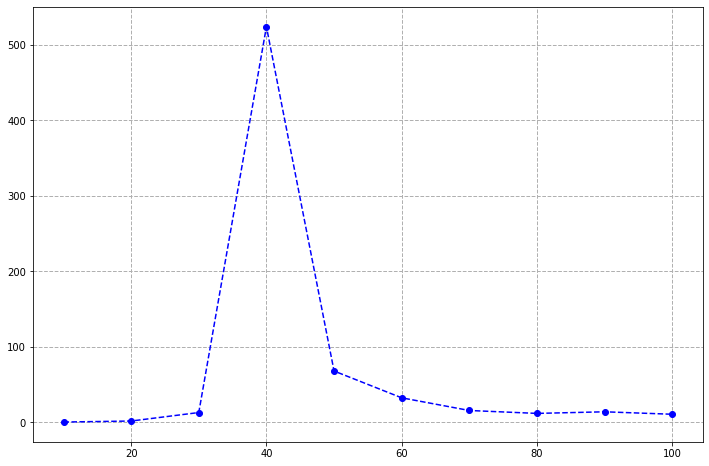
\includegraphics[width=0.45\textwidth]{../pictures/vr_cost_linear_gaussian.png}
\label{fig:subfig1}}
\qquad
\subfloat[Subfigure 2 list of figures text][$f(x)=\sum_{i=1}^d x^2_i$]{
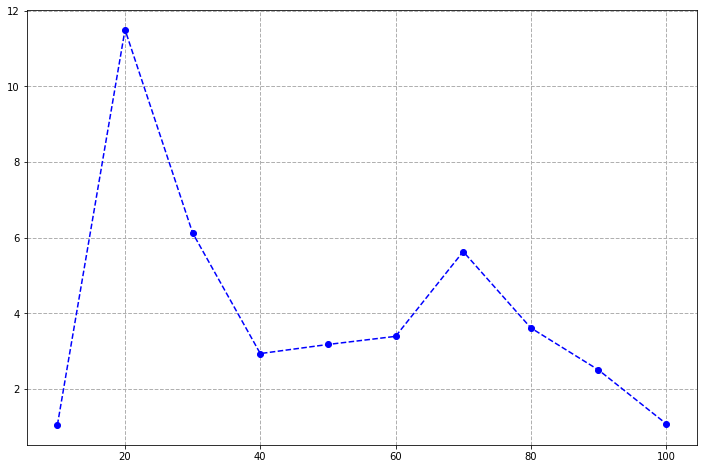
\includegraphics[width=0.45\textwidth]{../pictures/vr_cost_quadratic_gaussian.png}
\label{fig:subfig2}}
\caption{Cost-variance ratios \eqref{eq:cvR} as  functions of the truncation level $n_{\mathrm{trunc}}$ for  two-dimensional standard Gaussian distribution and different test functions.
\label{fig:gaus_cost}}
\end{figure}

\begin{figure}[tbh]
\centering
\subfloat[Subfigure 1 list of figures text][$f(x)=\sum_{i=1}^d x_i$]{
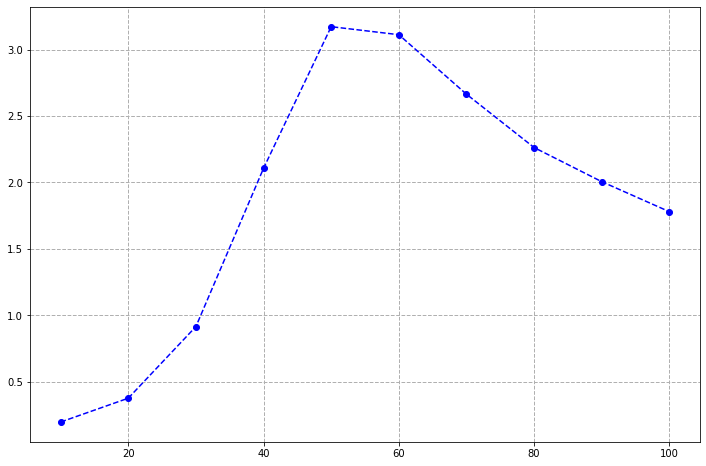
\includegraphics[width=0.45\textwidth]{../pictures/vr_cost_linear_gmm.png}
\label{fig:subfig1}}
\qquad
\subfloat[Subfigure 2 list of figures text][$f(x)=\sum_{i=1}^d x^2_i$]{
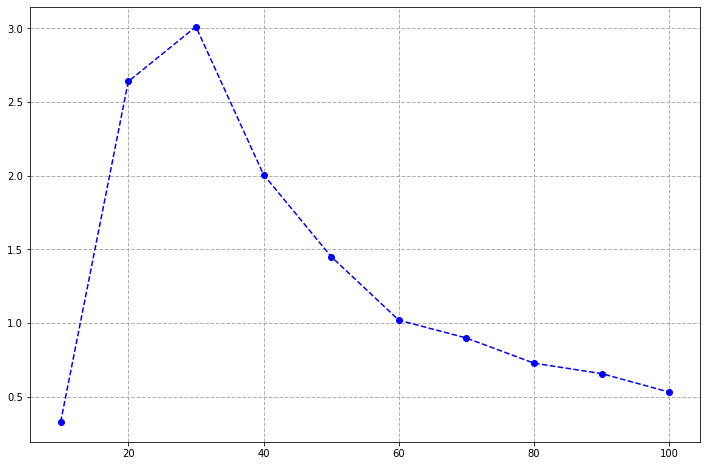
\includegraphics[width=0.45\textwidth]{../pictures/vr_cost_quadratic_gmm.png}
\label{fig:subfig2}}
\caption{Cost-variance ratios  \eqref{eq:cvR} as  functions of the truncation level $n_{\mathrm{trunc}}$ for a mixture of two-dimensional Gaussian distributions and different test functions.
\label{fig:gmm_cost}}
\end{figure}

\subsection{Gaussian mixtures}
 We consider  ULA with $\pi$  given by the mixture of two equally-weighted $d$-dimensional Gaussian distributions of the following form
\begin{eqnarray}
\label{eq:gmm}
\pi(x) = \frac{1}{2\sqrt{(2\pi)^{d}|\Sigma|}} \left( \rme^{-(1/2)(x-\mu)^T\Sigma^{-1}(x-\mu)} + \rme^{-(1/2)(x+\mu)^T\Sigma^{-1}(x+\mu)}\right)
\end{eqnarray}
where  $\mu \in \rset^d$, $\Sigma$ is a positive-definite $d \times d$ matrix and $|\Sigma|$ is its determinant. The function $U(x)$ and its gradient are given by
\[
U(x) = \frac{1}{2}(x-\mu)^T\Sigma^{-1}(x-\mu) - \ln{\left(1 + \rme^{-2\mu^\top \Sigma^{-1}x}\right)}
\]
and
\[
\nabla U(x) = \Sigma^{-1}(x-\mu) +2 \left(1 + \rme^{2 \mu^\top\Sigma^{-1} x}\right)^{-1} \Sigma^{-1}\mu ,
\]
respectively.
In our experiments we considered $d = 2$, $\mu = \left(0.5,0.5\right)$ and randomly generated positive-definite matrix $\Sigma$ (heterogeneous structure). In order to approximate the expectation \(\pi(f)\) with \(f(x)=\sum_{i=1}^d x_i\) or \(f(x) = \sum_{i=1}^d x^2_i\) we used constant step size $\gamma=0.1$ and sampled $\NtrainPath = 5 \times 10^4$ independent training trajectories, each one of size $n = 50$ with the burn-in period $n_{\text{burn}} = 100$. Then we solve the least squares  problems \eqref{eq:Qregr} using the first order polynomial approximations for $f(x)=\sum_{i=1}^d x_i$ and second order approximations for $f(x) = \sum_{i=1}^d x^2_i$ as described in the previous section. Hence we set $K = 1$ for $f(x)=\sum_{i=1}^d x_i$ or $K = 2$ for $f(x) = \sum_{i=1}^d x^2_i$. We set the truncation level \(n_{\mathrm{trunc}} = 50\). To test our variance reduction algorithm, we generated 100 independent trajectories of length $n = 2 \times 10^3$ and plot boxplots of the corresponding ergodic averages in Figure ~\ref{fig:GMM}. Our approach (MDCV, Martingale decomposition control variates) is compared to other variance reduction methods of \cite{mira2013zero} and \cite{belomestny2019esvm}. In the baselines we use first order polynomials in case of $K=1$ and second order polynomials for $K = 2$.
\par

 \begin{figure}[tbh]
\centering
\subfloat[Subfigure 1 list of figures text][$f(x)=\sum_{i=1}^d x_i$]{
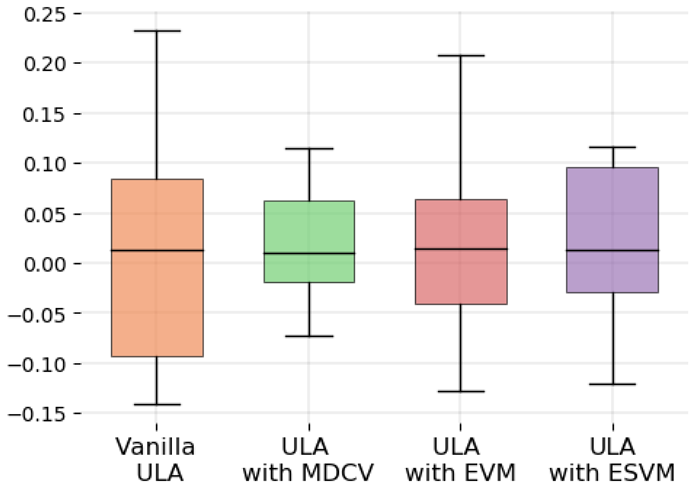
\includegraphics[width=0.45\textwidth]{../pictures/GMM_2d_lin_sum.png}
\label{fig:subfig1}}
\qquad
\subfloat[Subfigure 2 list of figures text][$f(x)=\sum_{i=1}^d x^2_i$]{
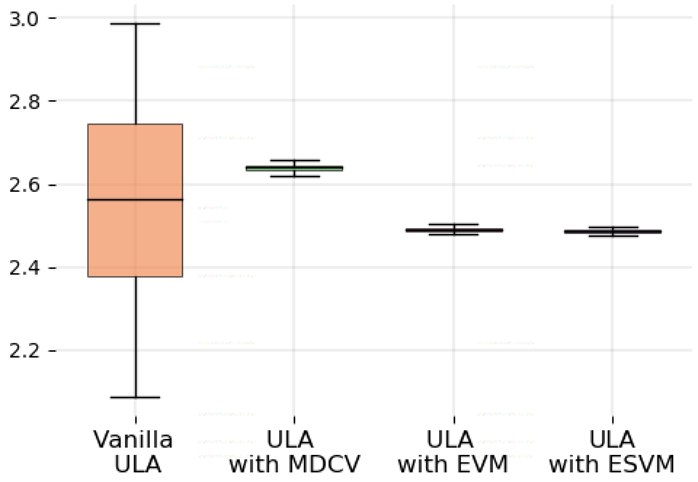
\includegraphics[width=0.45\textwidth]{../pictures/GMM_2d_lin_sum_squares.png}
\label{fig:subfig2}}
\caption{Boxplots of ergodic averages  from the variance reduced ULA algorithms for the Gaussian mixture model. The compared estimators are the ordinary empirical average  (Vanilla), our estimator of control variates (MDCV), zero variance estimator (ZV) and control variates obtained with empirical spectral variance minimisation (ESVM)
\label{fig:GMM}}
\end{figure}

%\begin{figure}[tbh]
%\centering
%\subfloat[Subfigure 1 list of figures text][$f(x)=\sum_{i=1}^d x_i$]{
%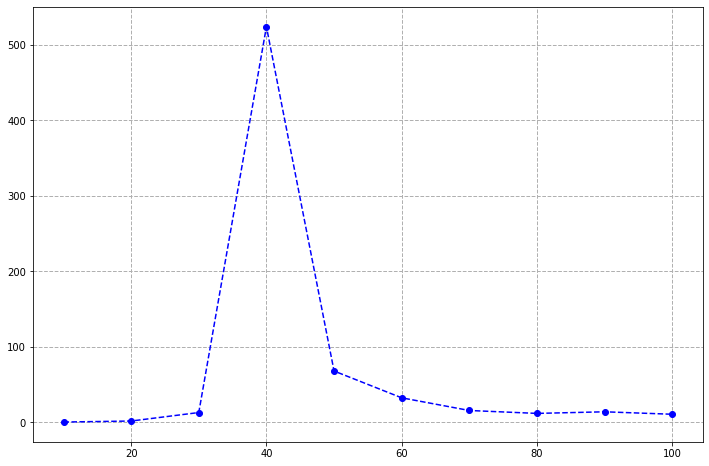
\includegraphics[width=0.45\textwidth]{../pictures/vr_cost_linear_gaussian.png}
%\label{fig:subfig3}}
%\qquad
%\subfloat[Subfigure 2 list of figures text][$f(x)=\sum_{i=1}^d x^2_i$]{
%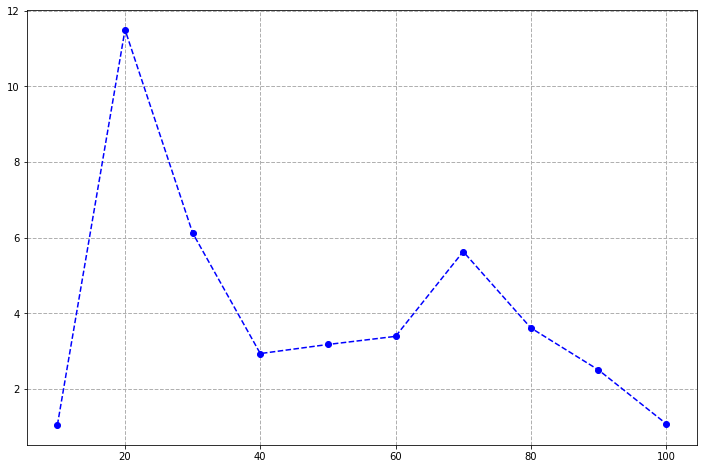
\includegraphics[width=0.45\textwidth]{../pictures/vr_cost_quadratic_gaussian.png}
%\label{fig:subfig4}}
%\caption{ Cost-variance ratios \eqref{eq:cvR} as  functions of the truncation level $n_{\mathrm{trunc}}$ for  two-dimensional standard Gaussian distribution and different test functions. \label{fig:G-costvar}}
%\end{figure}

%\begin{figure}[tbh]
%\centering
%\subfloat[Subfigure 1 list of figures text][$f(x)=\sum_{i=1}^d x_i$]{
%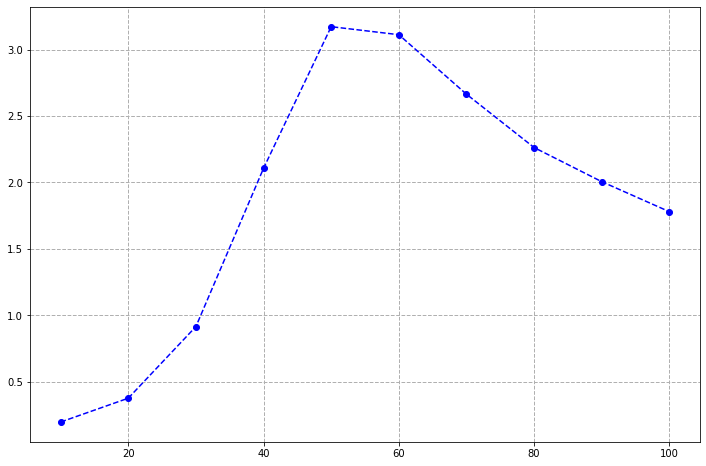
\includegraphics[width=0.45\textwidth]{../pictures/vr_cost_linear_gmm.png}
%\label{fig:subfig5}}
%\qquad
%\subfloat[Subfigure 2 list of figures text][$f(x)=\sum_{i=1}^d x^2_i$]{
%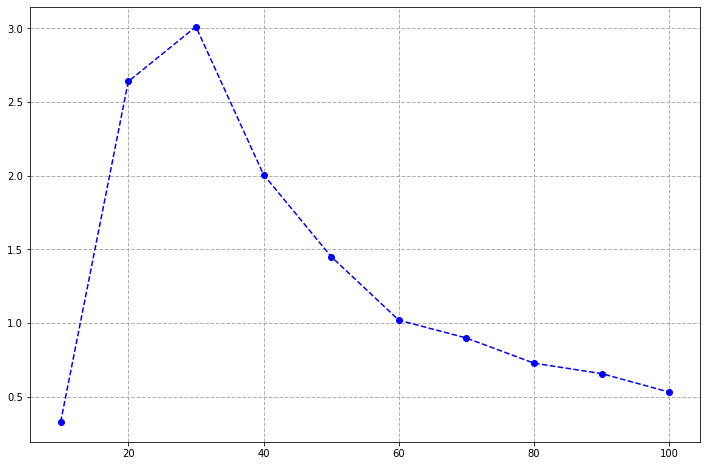
\includegraphics[width=0.45\textwidth]{../pictures/vr_cost_quadratic_gmm.png}
%\label{fig:subfig6}}
%\caption{ Cost-variance ratios  \eqref{eq:cvR} as  functions of the truncation level $n_{\mathrm{trunc}}$ for  a mixture of two-dimensional  Gaussian distribution and different test functions.
%\label{fig:GMM-costvar}}
%\end{figure}


\subsection{Banana shape distribution}
The “Banana-shape” distribution, proposed by \cite{haario1999adaptive}, can be obtained from a $d$-dimensional Gaussian vector with zero mean and covariance $\mathrm{diag}(p,1,\ldots,1)$ by applying transformation $\varphi_b(x) : \rset^d \rightarrow \rset^d$ of the form
\[
\varphi_b(x_1,\ldots,x_n) = (x_1, x_2 + bx^2_1 - pb,x_3,\ldots,x_d)
\]
where $p > 0$ and $b > 0$ are parameters; $b$ accounts for the curvature of density’s level sets. The potential $U$ is given by
\[
U(x_1,\ldots, x_d) = \frac{x_1^2}{2} + \frac{(x_2 + bx_1^2 - pb)^2}{2} + \frac{1}{2} \sum_{k=3}^{d} x_k^2 \eqsp.
\]
The quantity of interest is the expectation of $f(x) = x_2$. We set $p = 100, b = 0.1$ and consider $d=8$. We solve the least squares  problems \eqref{eq:Qregr} using the second-order polynomial approximations for the coefficients \(\hat{a}_{p,\mathbf{k}}\) as described in the previous section, hence we set $K = 2$. We use $T= 5 \times 10^4$ independent training trajectories, each of size $n=50$ with the burn-in $n_{\text{burn}} = 100$. We set the truncation level \(n_{\mathrm{trunc}} = 50\). To test our variance reduction algorithm, we generated 100 independent trajectories of length $n = 2 \times 10^3$ and display boxplots of the ergodic averages in Figure~\ref{fig:banana_shape}.

\begin{figure}[h]
\begin{center}
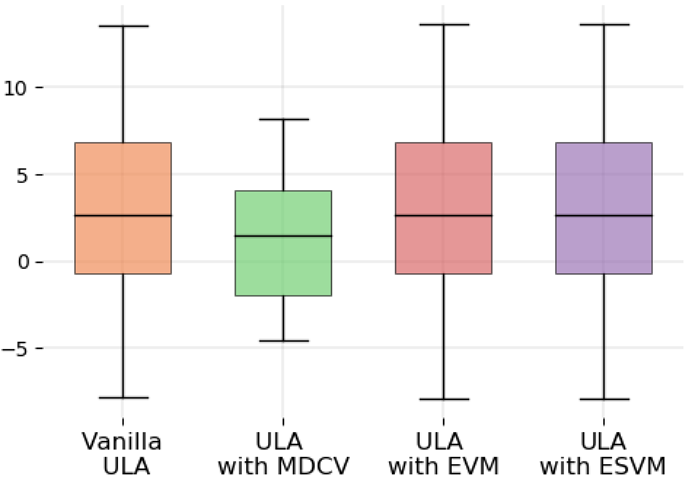
\includegraphics[width=0.6\textwidth]{../pictures/banana_shape.png}
\caption{Boxplots of ergodic averages  from the variance reduced ULA algorithms for the Banana shape density. The compared estimators are the ordinary empirical average (Vanilla), our estimator of control variates (MDCV), zero variance estimator (ZV) control variates obtained with empirical spectral variance minimisation (ESVM).
\label{fig:banana_shape}}
\end{center}
\end{figure}

\subsection{Binary Logistic Regression}
In this section, we consider  logistic regression. Let $\mathsf{Y} = \left(\mathsf{Y}_1,\ldots,\mathsf{Y}_n\right) \in \{0,1\}^m$ be binary response variables, $\mathsf{X} \in \rset^{m \times d}$ be a feature matrix and $\theta \in \rset^d$ - vector of regression parameters. We define log-likelihood of $i$-th observation as
\[
\ell(\mathsf{Y}_i | \theta, \mathsf{X}_i) = \mathsf{Y}_i \mathsf{X}_i^T\theta - \ln{(1 + \rme^{\mathsf{X}_i^T\theta})}
\]
In order to estimate $\theta$ according to given data, the Bayesian approach introduces prior distribution $\pi_0(\theta)$ and consider the posterior density $\pi(\theta| \mathsf{Y}, \mathsf{X})$ using Bayes' rule.

\begin{figure}[h]
\begin{center}
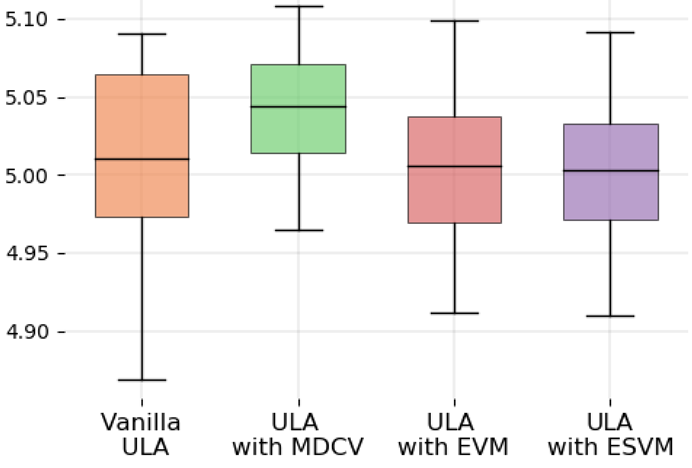
\includegraphics[width=0.6\textwidth]{../pictures/logreg_1st_order.png}
\caption{Boxplots of ergodic averages  from the variance reduced ULA algorithms for the Logistic Regression. The compared estimators are the ordinary empirical average (Vanilla), our estimator of control variates (MDCV), zero variance estimator (ZV) control variates obtained with empirical spectral variance minimisation (ESVM).
 \label{fig:2}}
\end{center}
\end{figure}

In the case of  Gaussian prior $\pi_0(\theta) \sim \mathcal{N}(0,\sigma^2 I_d)$, the unnormalized posterior density takes the form:
\begin{eqnarray*}
\pi(\theta | \mathsf{Y}, \mathsf{X}) \propto \exp \left\{ \mathsf{Y}^T \mathsf{X} \theta - \sum\limits_{i=1}^m \ln{\left(1 + \rme^{\mathsf{X}_i \theta}\right)} - \frac{1}{2\sigma^2} \left\|\theta\right\|_2^2 \right\},
\end{eqnarray*}
Thus we obtain
\begin{eqnarray*}
U(\theta) &=& -\mathsf{Y}^T \mathsf{X} \theta + \sum_{i=1}^m \ln{\left(1 + \rme^{\theta^T \mathsf{X}_i}\right)} + \frac{1}{2\sigma^2} \left\| \theta\right\|_2^2,
\\
\nabla U(\theta) &=& -\mathsf{Y}^T \mathsf{X} + \sum_{i=1}^m \frac{\mathsf{X}_i}{1 + \rme^{-\mathsf{\theta}^T \mathsf{X}_i}} + \frac{1}{\sigma^2} \theta.
\end{eqnarray*}
To demonstrate the performance of the proposed control variates approach in the above Bayesian logistic regression model, we take a simple dataset from \cite{mira2013zero}, which contains the measurements of four variables on $m=200$ Swiss banknotes. Prior distribution of the regression parameter $\mathbf{\theta} = \left( \theta_1, \theta_2, \theta_3, \theta_4 \right)$ assumed to be normal with the covariance matrix $\sigma^2 I_4$, where $\sigma^2 = 100$. To construct trajectories of length $n = 1 \times 10^4, $ we take step size $\gamma = 0.1$ for the ULA scheme with $N = 10^3$ burn-in steps. As in the previous experiment we use the first order polynomials approximations to analytically compute the coefficients $\hat{a}_{p-l,\mathbf{k}},$ based on $T = 10$ training trajectories. We put $n_{trunc} = 50$ and $K = 1$. The target function is taken to be $f(\theta) = \sum_{i=1}^{i=d}\theta_i$.  In order to test our variance reduction algorithm, we generate \(100\) independent test trajectories of length $n = 10^3$. In Figure ~\ref{fig:2} we compare our approach to the variance reduction methods of \cite{mira2013zero} and \cite{belomestny2019esvm}. In the baselines we use first order polynomials for the same reasons as in the Gaussian mixtures example.

\section{Proofs}
\label{sec:proofs}


\subsection{Proof of Theorem~\ref{thm:main-repr}}
The expansion obviously holds for $p = q=1$ and $j=0$.
Indeed, since $\left(\phi_{k}\right)_{k \geq 0}$ is a complete orthonormal system in \(L^2(\mathbb{R}^d, P_{\xi})\), it holds in \(L^2(\mathsf{P})\) that
\[
f(X^x_{1})=\PE[f(X^x_{1})]+\sum_{k\geq1}a_{1,1,k}(x)\phi_{k}(\xi_{1})
\]
for any bounded $f$ with $a_{1,1,k}(x)=\PE[f(X_{1}^x)\phi_{k}(\xi_{1})]$.
Assume now that (\ref{eq:mart_repr}) holds for some $m < p$, any $q \leq m$, $j < q \leq m$ and all bounded $f$. Let us prove that the induction assumption holds for $q=m+1$ and all $j < q$.
The orthonormality and completeness
of the system $\left(\phi_{k}\right)_{k=0}^\infty$ implies that for any bounded $f$ and $y \in \rset^d$,
$\lim_{n \rightarrow \infty}\Psi_{n,m+1,1}(y)= 0$ with $\Psi_{n,m+1,1}(y)= \PE[|f(X^y_{m,m+1}) - f_{n,m+1,1}(y)|^2]$ and
\[
f_{n,m+1,1}(y) = \PE[f(X^y_{m,m+1})] +  \sum\limits_{k=1}^{n}\PE[f(X^y_{m,m+1})\phi_{k}(\xi_{m+1})]\phi_k(\xi_{m+1}).
\]
Note that  for any $y \in \rset^d$ and $n \in \nset$ it holds $\Psi_{n,m+1,1}(y) \leq \Psi_{0,m+1,1}(y)$ and
\begin{eqnarray*}
\PE \left[ \psi_{0,m+1,1}(X_m^x) \right] &=& \PE \left[ \left. \PE \left[ \psi_{0,m+1,1}(X_m^x) \right| \mathcal{G}_m\right]\right] = \PE \left[ \left. \PE \left[ |f(X^{X_m^x}_{m,m+1}) - \PE f(X^{X_m^x}_{m,m+1})|^2 \right| X_m^x\right]\right]
\\
&=& \PE \left[ |f(X_{m+1}^x) - \PE f(X_{m+1}^x)|^2 \right] = \PVar{f(X_{m+1}^x)} < \infty
\end{eqnarray*}
Hence, by Lebesgue dominated convergence theorem, $\lim_{n \rightarrow \infty}\PE \left[\psi_{n,m+1,1}(X_m^x)\right] = 0$ and since for all $y \in \rset^d$ the expectation $\PE[f(X^y_{m,m+1})]$ is a version of $\PE \left[f(X^y_{m,m+1}) | \mathcal{G}_m \right]$, it holds in \(L^2(\mathsf{P})\) that
\begin{equation}
\label{eq:1-step-decomp}
f(X^x_{m+1}) = \PE[f(X^x_{m+1})|\mathcal{G}_m] + \sum\limits_{k=1}^{\infty}a_{m+1,m+1,k}(X^x_{m})\phi_{k}(\xi_{m+1})
\end{equation}
where
\[
a_{m+1,m+1,k}(y) = \PE \left[f(X^y_{m,m+1})\phi_k\left(\xi_{m+1}\right)\right]
\]
which is the required statement in the case $q = m+1$ and $j=m$.
Now assume that $j<m$.
Set $g(y) = \PE \left[f(X_{m,m+1}^y)\right]$. Note that $\mathsf{P}$-a.s. it holds $g(X_m^x) = \PE\left[\left.f(X_m^x) \right| \mathcal{G}_m\right]$ and $g$ is bounded by construction. Hence the induction hypothesis applies, and we get
\begin{equation}\label{eq:28082017a1}
\mathsf{E}\left[\left.f(X^x_{m+1})\right| \mathcal{G}_m \right]=\mathsf{E}\left[\left.f(X^x_{m+1})\right| \mathcal{G}_j \right]+\sum_{k\geq1}\sum_{l=j+1}^{m}a_{m+1,l,k}(X^x_{l-1})\phi_{k}(\xi_{l})
\end{equation}
with
\begin{align*}
a_{m+1,l,k}(X^x_{l-1}) &= \mathsf{E}\left[\left.\mathsf{E}\left[\left.f(X^x_{m+1})\right|\mathcal{G}_{m}\right]\phi_{k}(\xi_{l})\right|\mathcal{G}_{l-1}\right]
 = \mathsf{E}\left[\left.f(X^x_{m+1})\phi_{k}(\xi_{l})\right|X^x_{l-1}\right].
\end{align*}
where for $y \in \rset^d$,
\[
a_{m+1,l,k}(y) = \mathsf{E}\left[f(X^y_{l-1,m+1})\phi_{k}(\xi_{l})\right]
\]
Formulas \eqref{eq:1-step-decomp}
and~\eqref{eq:28082017a1} conclude the induction step for $q = m+1$ and all $j < q$ and hence the proof.


\subsection{Proof of Lemma~\ref{lem:variance}}
In the sequel, the notation $A(\gamma,n,x) \lesssim B(\gamma,n,x)$ means that there exist $\gamma_0 > 0$, and $C < \infty$ such that for all  $\gamma \in (0,\gamma_0]$, $x \in \rset^d$, $n \in \nset$, $A(\gamma,n,x) \leq C B(\gamma,n,x)$.

Under assumptions {\bf (H1)} and {\bf (H2)} the Markov chain $(X^x_{p})_{p \in \nset_0}$ is $V-$geometrically ergodic with $V(x) = 1+\|x\|^2$ and $\rho = \rme^{-\kappa\gamma}$ with $\kappa$ specified in Lemma~\ref{lem:v_ergodicity}. Due to lemma~\ref{lem:covariance},
\[
\PVar[\pi_n^N(f)]\lesssim \frac{1}{n(1-\rho^{1/2})}
\]
and the result of lemma follows from Taylor expansion of denominator.



\subsection{Proof of Theorem~\ref{th:mr}}
For $l\le p$ and $x \in \rset^d$, we have the representation
\[
X^x_{p}=G_{p}(x,\sqrt{\gamma}Z_{1},\ldots,\sqrt{\gamma}Z_{p}),
\]
where the function \(G_{p}:\) \(\mathbb{R}^{d\times(p+1)}\to \mathbb{R}^{d}\) is defined as
\begin{equation}
\label{eq:definition-G-p-l}
G_{p}(x,y_1,\ldots,y_p):=\Phi(\cdot,y_{p})\circ\Phi(\cdot,y_{p-1})\circ\ldots\circ\Phi(x,y_{1})
\end{equation}
with, for $x,y\in\mathbb R^d$,   $\Phi(x,y)=x-\gamma\mu(x)+y$.
As a consequence, for a function $f\colon\mathbb R^d\to\mathbb R$
as in Section~\ref{sec:setup}, we have
$$
f\left(X_{p}\right) =f\circ G_{p}(X_{0},\sqrt{\gamma}Z_{1},\ldots,\sqrt{\gamma}Z_{p}).
$$
In what follows, for $\mathbf{k}\in\mathbb N_0^d$,
we use the shorthand notation
\begin{equation}
\label{eq:definition-differential-f-p}
\partial_{1}^{\mathbf k} f\left(X_{p}\right)
:=\partial_{1}^{\mathbf k} [f\circ G_{p}](X_{0},\sqrt{\gamma}Z_{1},\ldots,\sqrt{\gamma}Z_{p})
\end{equation}
whenever the function $f\circ G_{p}$ is smooth enough
(that is, $f$ and $\mu$ need to be smooth enough).
Finally, for a multi-index $\mathbf{k}=(k_i)\in\mathbb N_0^d$, we use the notation
\(\mathbf{k} ! :=k_1!\cdot\ldots\cdot k_d !\)

\begin{lem}\label{eq:a_repr}
For any \(\mathbf{k},\mathbf{k}'\in \mathbb{N}_0^d\) such that \(\mathbf{k}'\le \mathbf{k}\) componentwise and $\| \mathbf{k}' \| \leq K$, the following representation holds
\[
\bar a_{p,\mathbf{k}}(x)=\left(\gamma^{|\mathbf{k}'|}\frac{(\mathbf{k}-\mathbf{k}') !}{\mathbf{k}!}\right)^{1/2}
\PE\left[
\partial_{1}^{\mathbf{k}'}f(X^x_p)\mathbf{H}_{\mathbf{k}-\mathbf{k}'}(Z_1)\right] \eqsp,
\]
where $\bar a_{p,\mathbf{k}}$ is defined in \eqref{eq:definition-bar-a}.
\end{lem}

\begin{proof}
Note that for the normalized Hermite polynomial $\mathbf H_{\mathbf k}$ on $\mathbb R^d$,
$\mathbf k\in\mathbb N_0^d$, it holds
$$
\mathbf{H}_{\mathbf{k}}(z)\boldsymbol{\varphi}(z)
=\frac{(-1)^{|\mathbf{k}|}}{\sqrt{\mathbf{k} !}} \partial^{\mathbf{k}} \boldsymbol{\varphi}(z).
$$
This enables to use the integration by parts in vector form as follows
(below $\prod_{j=l+1}^p:=1$ whenever $l=p$)
\begin{align*}
&\bar a_{p,\mathbf{k}}(x)
 =
\int_{\mathbb R^d}\ldots\int_{\mathbb R^d}
f\circ G_{p}(x,\sqrt{\gamma}z_{1},\ldots,\sqrt{\gamma}z_{p})
\mathbf{H}_{\mathbf{k}}(z_{1})\boldsymbol{\varphi}(z_1)
\prod_{j=2}^p\boldsymbol{\varphi}(z_j)\, \rmd z_{1}\ldots \rmd z_{p}
\\
& =
\frac{1}{\sqrt{\mathbf k!}}
\int_{\mathbb R^d}\ldots\int_{\mathbb R^d}
f\circ G_{p}(x,\sqrt{\gamma}z_{1},\ldots,\sqrt{\gamma}z_{p})
(-1)^{|\mathbf{k}|}\partial^{\mathbf{k}} \boldsymbol{\varphi}(z_1)
\prod_{j=2}^p\boldsymbol{\varphi}(z_j)\, \rmd z_{1}\ldots  \rmd z_{p}
\\
& =
\frac{\gamma^{|\mathbf k'|/2}}{\sqrt{\mathbf k!}}
\int_{\mathbb R^d}\ldots\int_{\mathbb R^d}
\partial_{1}^{\mathbf k'}[f\circ G_{p}](x,\sqrt{\gamma}z_{1},\ldots,\sqrt{\gamma}z_{p})
(-1)^{|\mathbf{k}-\mathbf k'|}\partial^{\mathbf{k}-\mathbf k'} \boldsymbol{\varphi}(z_1)
\prod_{j=2}^p\boldsymbol{\varphi}(z_j)\, \rmd z_{1}\ldots \rmd z_{p}
\\
 & =\gamma^{|\mathbf{k}'|/2}\frac{\sqrt{(\mathbf{k}-\mathbf{k}')!}}{\sqrt{\mathbf{k}!}}\mathsf{E}\left[\partial_{y_{1}}^{\mathbf{k}'}[f\circ G_{p}](x,\sqrt{\gamma}Z_{1},\ldots,\sqrt{\gamma}Z_{p})\mathbf{H}_{\mathbf{k}-\mathbf{k}'}(Z_{1})\right].
\end{align*}
The last expression yields the result.
\end{proof}

For multi-indices $\mathbf k,\mathbf k'\in\mathbb N_0^d$
with $\mathbf k'\le\mathbf k$ componentwise
and $\mathbf k'\ne\mathbf k$, $\| k' \| \leq K$,
we get applying first Lemma~\ref{eq:a_repr},
\begin{equation*}
A_{s,\mathbf{k}}(x)
=\left(\gamma^{|\mathbf{k}'|}\frac{(\mathbf{k}-\mathbf{k}')!}{\mathbf{k}!}\right)^{1/2}
\,
\PE\left[ \sum\nolimits_{r=1}^{s}\{\partial_{1}^{\mathbf{k}'} f(X^x_r)-\PE[\partial_{1}^{\mathbf{k}'}f(X^x_r)]\}\mathbf{H}_{\mathbf{k}-\mathbf{k}'}(Z_1)\right]
\end{equation*}
where $A_{s,\mathbf{k}}$ is defined in \eqref{eq:definition-A-s,k}.
Assume that $\mu$ and $f$ are $K\times d$ times continuously differentiable.
Then, given $\mathbf k\in\mathbb N_0^d$,
by taking $\mathbf k'= \mathbf k'(\mathbf k)
=K(\indiacc{k_1>K}\,\ldots, \indiacc{k_d>K})$, we get
\begin{multline}
\label{eq:sum_abar}
\sum_{\mathbf{k}\colon\|\mathbf{k}\|\geq K+1}A^2_{s,\mathbf{k}}(x)
=\sum_{\mathbf{k}\colon\|\mathbf{k}\|\geq K+1}\left(\gamma^{|\mathbf{k}'|}\frac{(\mathbf{k}-\mathbf{k}')!}{\mathbf{k}!}\right)Q_s(\mathbf{k}',\mathbf{k}-\mathbf{k}')\\
= \left\{ \sum_{I\subseteq\{1,\ldots,d\},\, I\neq \emptyset}\gamma^{|I|K}\sum_{\mathbf{m}_{I}\in\mathbb{N}_{I}^{d}}\frac{\mathbf{m}_{I}!}{\left(\mathbf{m}_{I}+\mathbf{K}_{I}\right)!} \right\}
\left\{ \sum_{\mathbf{m}_{I^c}\in \mathbb{N}^d_{0,I^c},\,\|\mathbf{m}_{I^c}\|\leq K}Q_s(\mathbf{\mathbf{K}}_{I},\mathbf{m}_{I}+\mathbf{m}_{I^c}) \right\},
\end{multline}
where for any two multi-indices \(\mathbf{r},\) \(\mathbf{q}\) from \(\mathbb{N}_0^d\)
\begin{equation*}
Q_s(\mathbf{r},\mathbf{q})
=
\left\{\PE\left[\sum_{p=1}^{s}\left\{\partial_{1}^{\mathbf r}f\left(X^x_{p}\right)-\PE\left[\partial_{1}^{\mathbf r}f\left(X^x_{p}\right)\right]\right\}\mathbf{H}_{\mathbf{q}}(Z_{1})\right]\right\}^{2}.
\end{equation*}
In \eqref{eq:sum_abar} the first sum runs over all nonempty subsets $I$ of the set $\{1,\ldots,d\}.$
For any subset $I,$ $\mathbb{N}_{I}^{d}$ stands for a set
of multi-indices $\mathbf{m}_{I}$ with elements $m_{i}=0,$ $i\not\in I,$
and $m_{i}\in\mathbb{N},$  $i\in I.$ Moreover, \(I^c=\{1,\ldots,d\}\setminus I\) and \(\mathbb{N}^d_{0,I^c}\) stands for a set
of multi-indices $\mathbf{m}_{I^c}$ with elements $m_{i}=0,$ $i\in I,$
and $m_{i}\in\mathbb{N}_0,$  $i\not\in I.$ Finally, the multi-index \(\mathbf{K}_I\) is defined as $\mathbf{\mathbf{K}}_{I}=(K1_{\{1\in I\}},\ldots,K1_{\{d\in I\}}).$
Applying the estimate
\begin{eqnarray*}
\frac{\mathbf{m}_{I}!}{\left(\mathbf{m}_{I}+\mathbf{K}_{I}\right)!}\leq (1/2)^{|I| K},
\end{eqnarray*}
we get
\begin{align}
\label{eq:sumA}
\sum_{\mathbf{k}\colon\|\mathbf{k}\|\geq K+1}A^2_{s,\mathbf{k}}(x)
&\leq
\sum_{I\subseteq\{1,\ldots,d\},\, I\neq \emptyset} (\gamma/2)^{|I|K}
\\
\nonumber
& \times\sum_{\mathbf{m}_{I}\in\mathbb{N}_{I}^{d}} \sum_{\mathbf{m}_{I^c}\in \mathbb{N}^d_{0,I^c},\,\|\mathbf{m}_{I^c}\|\leq K} Q(\mathbf{\mathbf{K}}_{I},\mathbf{m}_{I}+\mathbf{m}_{I^c})
\\
\nonumber
&\leq
\sum_{I\subseteq\{1,\ldots,d\},\, I\neq \emptyset} (\gamma/2)^{|I|K} \sum_{\mathbf{m}\in\mathbb{N}_0^{d}} Q(\mathbf{\mathbf{K}}_{I},\mathbf{m}).
\end{align}
The Parseval identity implies that for any function $\varphi: \rset^d \to \rset$ satisfying $\PE[\varphi^2(Z_1)] < \infty$,
\[
\sum_{\mathbf{m}\in \nset^d_0} \{\PE[\varphi(Z_1) \mathbf{H}_\mathbf{m}(Z_1)] \}^2 \le \PE[\{\varphi(Z_1)\}^2]
\]
Using this identity in \eqref{eq:sumA} implies
\begin{eqnarray*}
\sum_{\mathbf{k}\colon\|\mathbf{k}\|\geq K+1}A^2_{s,\mathbf{k}}(x)
&\leq & \sum_{I\subseteq\{1,\ldots,d\},\, I\neq \emptyset}
\left(\frac{\gamma}{2}\right)^{|I|K}
\PVar\left(\sum_{p=1}^{s}\partial_{1}^{\mathbf{K}_I}f\left(X^x_{p}\right)
\right)
\end{eqnarray*}
Next we show that under the conditions  of Theorem~\ref{th:mr}
\begin{eqnarray*}
\PVar\left(\sum_{p=1}^{q}\partial_{1}^{\mathbf{K}_I}f\left(X^x_{p}\right)
\right)\leq C\gamma^{-1} \rme^{\varkappa n\gamma^2}(1+V(x)),\quad q=1,\ldots,n,
\end{eqnarray*}
for all $x$ and some constants $C,\varkappa>0$  not depending on $n$ and $\gamma.$
To keep the notational burden at a reasonable level, we present the proof only in one-dimensional case.
Multidimensional extension is straightforward but requires involved notations.
First, we need to prove several auxiliary results.
\begin{lem}\label{lem:06062018a1}
Let $(x_p)_{p\in\mathbb N_0}$
and $(\epsilon_p)_{p\in\mathbb N}$
be sequences of nonnegative real numbers
satisfying $x_0=\ol C_0$ and
\begin{align}
0&\le x_p\le\alpha_p x_{p-1}+\gamma \epsilon_p,\quad p\in\mathbb N,
\label{eq:06062018a1}\\
0&\le\epsilon_p\le\ol C_1\prod_{k=1}^p \alpha_k^2,\quad p\in\mathbb N,
\label{eq:06062018a2}
\end{align}
where $\alpha_p,\gamma\in(0,1)$, $p\in\mathbb N$,
and $\ol C_0,\ol C_1$ are some nonnegative constants. Assume
\begin{equation}\label{eq:06062018a3}
\gamma \sum_{r=1}^\infty \prod_{k=1}^r \alpha_k\le\ol C_2
\end{equation}
for some constant $\ol C_2$. Then
$$
x_p\le(\ol C_0+\ol C_1\ol C_2)\prod_{k=1}^p \alpha_k,\quad p\in\mathbb N.
$$
\end{lem}

\begin{proof}
Applying~\eqref{eq:06062018a1} recursively, we get
$$
x_p\le\ol C_0\prod_{k=1}^p \alpha_k
+\gamma\sum_{r=1}^p \epsilon_r
\prod_{k=r+1}^p \alpha_k,
$$
where we use the convention $\prod_{k=p+1}^p:=1$.
Substituting estimate~\eqref{eq:06062018a2}
into the right-hand side, we obtain
$$
x_p\le\left(\ol C_0+\ol C_1
\gamma\sum_{r=1}^p  \prod_{k=1}^r \alpha_k
\right)
\prod_{k=1}^p \alpha_k,
$$
which, together with~\eqref{eq:06062018a3}, completes the proof.
\end{proof}
In what follows, we use the notation
\begin{equation}
\label{eq:definition-alpha}
\alpha_k=1-\gamma \mu'(X_{k-1}^x),\quad k\in\mathbb N.
\end{equation}
The assumption \eqref{eq:smooth-mu} implies that  $|\mu'(x)|\leq B_\mu$ for some constant $B_\mu>0$ and all $x\in \mathbb{R}^d$. Without loss of generality we suppose that $\gamma B_\mu<1.$
\begin{lem}\label{lem:06062018a2}
Under assumptions of Theorem~\ref{th:mr},
for all natural $r\le K$ and $l\le p$, there exist constants $C_r$ (not depending on $l$ and $p$) such that
\begin{equation}
\label{eq:08062018b2}
\left|\partial_{y_l}^r X^x_p \right| \le C_r\prod_{k=l+1}^p (1-\gamma\mu'(X^x_{k-1}))\quad \text{a.s.}
\end{equation}
where $\partial_{y_l}^r X^x_p$ is defined in \eqref{eq:definition-differential-f-p}. Moreover, we can choose $C_1=1$.
\end{lem}
\begin{lem}\label{lem:06062018a3}
Under assumptions of Theorem~\ref{th:mr},
for all natural $r\le K$, $j\ge l$ and $p>j$, we have
\begin{equation}\label{eq:08062018b3}
\left|\partial_{y_j} \partial_{y_l}^r X^x_p\right|
\le c_r\prod_{k=l+1}^p (1-\gamma\mu'(X^x_{k-1})), \quad \text{a.s.}
\end{equation}
with some constants $c_r$
not depending on $j$, $l$ and $p$,
while, for $p\le j$, it holds
$\partial_{y_{j}}\partial_{y_{l}}^{r}X^x_{p}=0$.
\end{lem}

\begin{proof}
The last statement is straightforward.
We fix natural numbers $j\ge l$ and prove~\eqref{eq:08062018b3}
for all $p>j$ by induction in~$r$.
First, for $p>j$, we write
$$
\partial_{y_{l}}X^x_{p}
=\left[1-\gamma\mu'(X^x_{p-1})\right]\partial_{y_{l}}X^x_{p-1}
$$
and differentiate this identity with respect to~$y_j$
$$
\partial_{y_{j}}\partial_{y_{l}}X^x_{p}
=\left[1-\gamma\mu'(X^x_{p-1})\right]\partial_{y_{j}}\partial_{y_{l}}X^x_{p-1}-\gamma\mu''(X^x_{p-1})\partial_{y_{j}}X^x_{p-1}\partial_{y_{l}}X^x_{p-1}.
$$
By Lemma~\ref{lem:06062018a2}, we have
\begin{align*}
|\partial_{y_{j}}\partial_{y_{l}}X^x_{p}|
&\le\alpha_p|\partial_{y_{j}}\partial_{y_{l}}X^x_{p-1}|
+\gamma
B_\mu
\prod_{k=l+1}^{p-1}\alpha_k
\prod_{k=j+1}^{p-1}\alpha_k\\
&\le\alpha_p|\partial_{y_{j}}\partial_{y_{l}}X^x_{p-1}|
+\gamma
\const
\prod_{k=l+1}^{j}\alpha_k
\prod_{k=j+1}^{p}\alpha_k^2,
\quad p\ge j+1,
\end{align*}
with a suitable constant.
By Lemma~\ref{lem:06062018a1} applied
to bound $|\partial_{y_{j}}\partial_{y_{l}}X^x_{p}|$
for $p\ge j+1$
(notice that $\partial_{y_j}\partial_{y_l}X^x_j=0$, that is,
$\ol C_0$ in Lemma~\ref{lem:06062018a1} is zero,
while $\ol C_1$ in Lemma~\ref{lem:06062018a1}
has the form $\const\prod_{k=l+1}^j \alpha_k$),
we obtain~\eqref{eq:08062018b3} for $r=1$.
The induction hypothesis is now that the inequality
\begin{equation}\label{eq:induc-derive}
\left|\partial_{y_{j}}\partial_{y_{l}}^{k}X^x_{p}\right|
\leq c_{k}\prod_{s=l+1}^{p}\alpha_{s}
\end{equation}
holds for all natural $k<r\;(\le K)$ and $p>j$.
We need to show~\eqref{eq:induc-derive} for $k=r$.
Fa\`a di Bruno's formula implies for $2\le r\le K$ and $p>l$
\begin{align}
\partial_{y_{l}}^{r}X^x_{p}
&=\left[1-\gamma\mu'(X^x_{p-1})\right]\partial_{y_{l}}^{r}X^x_{p-1}
\label{eq:08062018a1}\\
&\hspace{1em}-\gamma\sum\frac{r!}{m_{1}!\ldots m_{r-1}!\,}\mu^{(m_{1}+\ldots+m_{r-1})}(X^x_{p-1})\prod_{k=1}^{r-1}\left(\frac{\partial_{y_{l}}^{k}X^x_{p-1}}{k!}\right)^{m_{k}},
\notag
\end{align}
where the sum is taken over all $(r-1)$-tuples of nonnegative integers
$(m_{1},\ldots,m_{r-1})$ satisfying the constraint
\begin{equation}\label{eq:09062018a1}
1\cdot m_{1}+2\cdot m_{2}+\ldots+(r-1)\cdot m_{r-1}=r.
\end{equation}
Notice that we work with $(r-1)$-tuples
rather than with $r$-tuples
because the term containing
$\partial_{y_l}^r X^x_{p-1}$
on the right-hand side of~\eqref{eq:08062018a1}
is listed separately.
For $p>j$, we then have
\begin{align}
&\partial_{y_{j}}\partial_{y_{l}}^{r}X^x_{p}
=\left[1-\gamma_{p}\mu'(X^x_{p-1})\right]\partial_{y_{j}}\partial_{y_{l}}^{r}X^x_{p-1}-\gamma\mu''(X^x_{p-1})\partial_{y_{l}}^{r}X^x_{p-1}\partial_{y_{j}}X^x_{p-1}
\label{eq:09062018a2}\\
&\hspace{1em}-\gamma\sum\frac{r!}{m_{1}!\ldots m_{r-1}!\,}\mu^{(m_{1}+\ldots+m_{r-1}+1)}(X^x_{p-1})\partial_{y_{j}}X^x_{p-1}\prod_{k=1}^{r-1}\left(\frac{\partial_{y_{l}}^{k}X^x_{p-1}}{k!}\right)^{m_{k}}
\notag\\
&\hspace{1em}-\gamma\sum\frac{r!}{m_{1}!\ldots m_{r-1}!\,}\mu^{(m_{1}+\ldots+m_{r-1})}(X^x_{p-1})\partial_{y_{j}}\left[\prod_{k=1}^{r-1}\left(\frac{\partial_{y_{l}}^{k}X^x_{p-1}}{k!}\right)^{m_{k}}\right]
\notag\\
&\hspace{1em} =\left[1-\gamma\mu'(X^x_{p-1})\right]\partial_{y_{j}}\partial_{y_{l}}^{r}X^x_{p-1}+\gamma\epsilon_{l,j,p},
\notag
\end{align}
where the last equality defines the quantity $\epsilon_{l,j,p}$.
Furthermore,
\begin{eqnarray*}
\partial_{y_{j}}\left[\prod_{k=1}^{r-1}\left(\frac{\partial_{y_{l}}^{k}X^x_{p-1}}{k!}\right)^{m_{k}}\right]&=&\sum_{s=1}^{r-1}\frac{m_{s}}{s!}\left(\frac{\partial_{y_{l}}^{s}X^x_{p-1}}{s!}\right)^{m_{s}-1}\partial_{y_{j}}\partial_{y_{l}}^{s}X^x_{p-1}
\\
&& \times \prod_{k\le r-1,\,k\neq s}\left(\frac{\partial_{y_{l}}^{k}X^x_{p-1}}{k!}\right)^{m_{k}}.
\end{eqnarray*}
Using Lemma~\ref{lem:06062018a2},
induction hypothesis~\eqref{eq:induc-derive}
and the fact that $m_{1}+\ldots+m_{r-1}\ge2$
for $(r-1)$-tuples of nonnegative integers
satisfying~\eqref{eq:09062018a1},
we can bound $|\epsilon_{l,j,p}|$ as follows
\begin{align*}
&\left|\epsilon_{l,j,p}\right|  \leq  B_{\mu}C_{r}\prod_{k=l+1}^{p-1}\alpha_{k}\prod_{k=j+1}^{p-1}\alpha_{k}+B_{\mu}\sum\frac{r!}{m_{1}!\ldots m_{r-1}!\,}\left[\prod_{k=j+1}^{p-1}\alpha_{k}\right]
\\
&\times \prod_{s=1}^{r-1}\left(\frac{C_{s}\prod_{k=l+1}^{p-1}\alpha_{k}}{s!}\right)^{m_{s}}\\
&+B_{\mu}\sum\frac{r!}{m_{1}!\ldots m_{r-1}!\,}\sum_{t=1}^{r-1}\frac{m_t}{t!}\left(\frac{C_{t}\prod_{k=l+1}^{p-1}\alpha_{k}}{t!}\right)^{m_{t}-1}c_t\left[\prod_{k=l+1}^{p-1}\alpha_{k}\right]
\\
&\times \prod_{s\le r-1,\,s\neq t}\left(\frac{C_{s}\prod_{k=l+1}^{p-1}\alpha_{k}}{s!}\right)^{m_{s}}\leq \const\prod_{k=l+1}^{j}\alpha_{k}\prod_{k=j+1}^{p}\alpha_{k}^{2}
\end{align*}
with some constant ``$\const$'' depending on
$B_\mu,r,C_1,\ldots,C_r,c_1,\ldots,c_{r-1}$.
Thus, \eqref{eq:09062018a2} now implies
$$
|\partial_{y_{j}}\partial_{y_{l}}^{r}X^x_{p}|
\le\alpha_p|\partial_{y_{j}}\partial_{y_{l}}^{r}X^x_{p-1}|
+\gamma \,\const\prod_{k=l+1}^{j}\alpha_{k}\prod_{k=j+1}^{p}\alpha_{k}^{2},
\quad p\ge j+1.
$$
We can again apply Lemma~\ref{lem:06062018a1}
to bound $|\partial_{y_{j}}\partial_{y_{l}}^r X^x_{p}|$
for $p\ge j+1$
(notice that $\partial_{y_j}\partial_{y_l}^r X^x_j=0$, that is,
$\ol C_0$ in Lemma~\ref{lem:06062018a1} is zero,
while $\ol C_1$ in Lemma~\ref{lem:06062018a1}
has the form $\const\prod_{k=l+1}^j \alpha_k$),
and we obtain~\eqref{eq:induc-derive} for $k=r$.
This concludes the proof.
\end{proof}

\begin{lem}
\label{lem:var_poincare}
Under assumptions of Theorem~\ref{th:mr}, it holds
$$
\mathsf{Var}\left[\sum_{p=1}^{q}\partial_{y_{1}}^{K}f\left(X_{p}^x\right)\right]\le  \gamma^{-1} C \rme^{\varkappa n\gamma^2}(1+V(x)), \quad q=1,\ldots,n,
$$
where $C,\varkappa>0$ are constants that do not depend on $n$ and $\gamma.$
\end{lem}
\begin{proof}
The expression
$\sum_{p=1}^q \partial_{y_1}^K f(X_p^x)$
can be viewed as a deterministic function of
$x,Z_1,Z_{2},\ldots,Z_q$
$$
\sum_{p=1}^q  \partial_{y_1}^K f(X_p^x)
=F(x,Z_1,Z_{2},\ldots,Z_q).
$$
By the (conditional) Gaussian Poincar\'e inequality,
we have
$$
\mathsf{Var}\left[\sum_{p=1}^{q}\partial_{y_{1}}^{K}f\left(X_{p}^x\right)\right]
\le\mathsf E_x\left[
\|\nabla_Z F(x,Z_1,Z_{2},\ldots,Z_q)\|^2
\right],
$$
where $\nabla_Z F=(\partial_{Z_1} F,\ldots,\partial_{Z_q} F)$,
and $\|\cdot\|$ denotes the Euclidean norm.
Notice that \(\partial_{Z_j} F=\sqrt{\gamma}\,\partial_{y_j} F\) and
hence
$$
\mathsf{Var}\left[\sum_{p=1}^{q}\partial_{y_{1}}^{K}f\left(X_{p}^x\right)\right]\leq\gamma^2\sum_{j=1}^{q}\mathsf{E}\left[\left(\sum_{p=1}^{q}\partial_{y_{j}}\partial_{y_{1}}^{K}f\left(X_{p}^x\right)\right)^{2}\right].
$$
It is straightforward to check that
$\partial_{y_j}\partial_{y_1}^K f(X_p^x)=0$
whenever $p<j$. Therefore, we get
\begin{equation}\label{eq:10062018a2}
\mathsf{Var}\left[\sum_{p=1}^{q}\partial_{y_{1}}^{K}f\left(X_{p}^x\right)\right]\leq\gamma^2\sum_{j=1}^{q}\mathsf{E}\left[\left(\sum_{p=j}^{q}\partial_{y_{j}}\partial_{y_{1}}^{K}f\left(X_{p}^x\right)\right)^{2}\right].
\end{equation}
Now fix $p$ and $j$, $p\ge j$, in $\{1,\ldots,q\}$.
By Fa\`a di Bruno's formula
\[
\partial_{y_{1}}^{K}f\left(X_{p}^x\right)=\sum\frac{K!}{m_{1}!\ldots m_{K}!}f^{(m_{1}+\ldots+m_{K})}(X_{p}^x)\prod_{k=1}^{K}\left(\frac{\partial_{y_{1}}^{k}X^x_{p}}{k!}\right)^{m_{k}},
\]
where the sum is taken over all $K$-tuples of nonnegative integers
$(m_1,\ldots,m_K)$ satisfying
$$
1\cdot m_{1}+2\cdot m_{2}+\ldots+K\cdot m_{K}=K.
$$
Then
\begin{eqnarray*}
\partial_{y_{j}}\partial_{y_{1}}^{K}f\left(X_{p}^x\right)
&=&\sum\frac{K!}{m_{1}!\ldots m_{K}!}f^{(m_{1}+\ldots+m_{K}+1)}(X^x_{p})\left[\partial_{y_{j}}X^x_{p}\right]\prod_{k=1}^{K}\left(\frac{\partial_{y_{1}}^{k}X_{p}^x}{k!}\right)^{m_{k}} \\
&&+\sum\frac{K!}{m_{1}!\ldots m_{K}!}f^{(m_{1}+\ldots+m_{K})}(X^x_{p})
\sum_{s=1}^{K}\frac{m_{s}}{s!}
\left(\frac{\partial_{y_{1}}^{s}X^x_{p}}{s!}\right)^{m_{s}-1}
\\
&& \times\left[\partial_{y_{j}}\partial_{y_{1}}^{s}X^x_{p}\right]
\prod_{k\le K,\,k\neq s}\left(\frac{\partial_{y_{1}}^{k}X^x_{p}}{k!}\right)^{m_{k}}.
\end{eqnarray*}
Using the bounds of
Lemmas \ref{lem:06062018a2} and~\ref{lem:06062018a3},
we obtain
\begin{eqnarray}
\label{eq:part-part}
\left|\partial_{y_{j}}\partial_{y_{1}}^{K}f\left(X_{p}^x\right)\right|
\leq A_{K}\prod_{k=2}^{p}\alpha_{k}
\end{eqnarray}
with a suitable constant $A_{K}$.
Substituting this in~\eqref{eq:10062018a2},
we proceed as follows
\begin{align*}
\mathsf{Var}_x\left[\sum_{p=1}^{q}\partial_{y_{1}}^{K}f\left(X_{p}^x\right)\right]
&\le
\gamma^2 A_{K}^{2}\sum_{j=1}^{q}
\mathsf{E}\left(\sum_{p=j}^{q}\prod_{k=2}^{p}\alpha_{k}\right)^{2}
\\
&\le
\frac{\gamma^2 A_{K}^{2}}{(1-\gamma B_\mu)^2}
\mathsf{E}\sum_{j=1}^{q}
\left(\sum_{p=j+1}^{q+1}  \prod_{k=2}^{p} \alpha_{k}
\right)^{2}
\\
%&=
%\frac{A_{K}^{2}}{(1-\gamma_1 b_\mu)^2}
%\sum_{j=l}^{q} \gamma_{j}
%\prod_{k=l+1}^{j} \alpha_{k}^2
%\left(
%\sum_{p=j+1}^{q+1} \gamma_{p} \prod_{k=j+1}^{p} \alpha_{k}
%\right)^{2}
%\\
&\le
\frac{\gamma^2 A_{K}^{2}}{(1-\gamma B_\mu)^3}
\mathsf{E}\sum_{j=1}^{q}
\prod_{k=1}^{j} \alpha_{k}
\left(\sum_{p=j+1}^{q+1}  \prod_{k=j+1}^{p} \alpha_{k}
\right)^{2}
\end{align*}

Now, from the H\"older inequality, we obtain (with $\|X\|_p = (\mathsf{E}X^p)^{\frac{1}{p}}$)
\begin{align*}
\mathsf{E}\left[\sum_{j=1}^{q}\prod_{k=l}^{j}\alpha_{k}\left( \sum_{p=j+1}^{q+1}\prod_{k=j+1}^{p}\alpha_{k}\right)^{2}\right] & \leq\sum_{j=1}^{q}\left\Vert \prod_{k=1}^{j}\alpha_{k}\right\Vert _{2}\left\Vert \sum_{p=j+1}^{q+1} \prod_{k=j+1}^{p}\alpha_{k}\right\Vert _{4}^{2}\\
 & \leq\sum_{j=1}^{q} \left\Vert \prod_{k=1}^{j}\alpha_{k}\right\Vert _{2}\left(\sum_{p=j+1}^{q+1}\left\Vert \prod_{k=j+1}^{p}\alpha_{k}\right\Vert _{4}\right)^{2}.
\end{align*}
Now using the fact that $\prod\limits_{k=j+1}^{p}\alpha_{k} \leq \exp\left(-\sum\limits_{k=j+1}^{p}\gamma\mu'(X_{k-1}^x)\right),$
we get
\[
\mathsf{E}\left[\sum_{j=1}^{q}\prod_{k=1}^{j}\alpha_{k}\left(\sum_{p=j+1}^{q+1}\prod_{k=j+1}^{p}\alpha_{k}\right)^{2}\right]\leq\sum_{j=1}^{q} \zeta^{1/2}_{1,j}(2) \left(\sum_{p=j+1}^{q+1} \zeta^{1/4}_{j+1,p}(4)\right)^{2},
\]
where we denote
\[
\zeta_{l,j}(u)=\mathsf{E}\left[\rme^{-u\gamma\sum_{k=l}^{j}\mu'(X^x_{k-1})}\right],\quad u>0.
\]
Note that $\mu^{\prime}(x)$ is bounded due  our assumptions and from \cite[Theorem~1]{delyon1999small} and Lemma~\ref{lem:v_ergodicity} in Appendix~\ref{sec:appendix} it follows that
\[
\mathsf{E}\left[\rme^{-u\gamma\left(\sum_{k=l}^{j}[\mu'(X^x_{k-1})-\pi_\gamma(\mu')]\right)}\right]\leq C_1 \rme^{\varkappa n\gamma^2}(1+V(x)),\quad u\gamma\leq \gamma_0,
\]
for some constants $\gamma_0$ and $C_1,\varkappa>0$. Then we have
\[
\zeta_{l,j}(u)=\mathsf{E}\left[\rme^{-s\gamma\sum_{k=l}^{j}\mu'(X^x_{k-1})}\right]\leq  C_1 \rme^{\varkappa n\gamma^2}(1+V(x)) \rme^{-s\gamma (j-l+1)\pi_\gamma(\mu')}.
\]
Furthermore, since $\mu\pi',\mu'\pi\in L^{1}(\mathbb{R})$ and $\pi^{\prime}(x) = -\frac{1}{2}\pi(x)\mu(x)$, we have
\[
\pi(\mu')=\int\mu'(x)\pi(x)\,dx=-\int\mu(x)\pi'(x)\,dx=\frac{1}{2}\int\mu^{2}(x)\pi(x)\,dx>0
\]
Note also that \(\pi_\gamma(\mu^{\prime}) \geq \pi_\gamma(\mu^{\prime}) - C_2\sqrt{\gamma}\)
yielding the bound
\[
\zeta_{l,j}(s) \leq  C_1 \rme^{\varkappa n\gamma^2}(1+V(x)) \rme^{-s\gamma(j-l+1)\alpha}
\]
where $ \alpha = \frac{1}{2}\int \mu^2(x)\pi(x)\,dx - C_1\sqrt{\gamma} > 0$ for sufficiently small $\gamma$. Hence we obtain
\begin{align*}
\sum_{p=j+1}^{q+1} \zeta^{1/4}_{j+1,p}(4) &\leq (C_1 \rme^{\varkappa n\gamma^2}(1+V(x)))^{1/4}\sum_{p=j+1}^{q+1} \rme^{-\gamma(p-j)\alpha}
\\
&\leq  (C_1 \rme^{\varkappa n\gamma^2}(1+V(x)))^{1/4}\frac{1}{1- \rme^{- \gamma\alpha}}
\end{align*}
and
\begin{align*}
\sum_{j=1}^{q} \zeta^{1/2}_{1,j}(2) \leq (C_1 \rme^{\varkappa n\gamma^2}(1+V(x)))^{1/2}\sum_{j=0}^{q} \rme^{-\gamma j\alpha}
\\
\leq  (C_1 \rme^{\varkappa n\gamma^2}(1+V(x)))^{1/2}\frac{ 1}{1- \rme^{- \gamma\alpha}}.
\end{align*}
Thus the final bound follows:
\begin{align*}
\mathsf{Var}\left[\sum_{p=1}^{q}\partial_{y_{1}}^{K}f\left(X^x_{p}\right)\right] \leq \gamma^{-1} C_K \rme^{\varkappa n\gamma^2} (1+V(x))
\end{align*}
 with $C_K$  depending neither on $q$ nor on $\gamma$. The proof is completed.
\end{proof}


\appendix
\section{Bounds for moments of  ULA}\label{sec:appendix}


\begin{definition}
\label{def:v_ergodicity}
Let $(X_p)_{p \in \nset_0}$ be a Markov chain taking values in some space $X$ with the Markov kernel $Q$ and stationary distribution $\pi$. We say that $(X_p)_{p \in \nset_0}$ is $V-$geometrically ergodic for a given function $V: X \rightarrow [1; +\infty)$ if there exist real numbers $C > 0$ and $0 < \rho < 1$ such that for any $n \in \nset$,
\begin{equation}
\label{eq:v_ergodicity}
d_V(\delta_xQ^{1,n},\pi) \leq C\rho^n V(x)
\end{equation}
\end{definition}

In all the sequel, without loss of generality, we assume that $\nabla U(0)=0$ and we set
\begin{equation}
\label{eq:definition-V}
V(x) = 1 + \|x\|^2 \eqsp.
\end{equation}
\begin{lem}
  \label{lem:quadratic_behaviour}
  Assume {\bf (H1)} and {\bf (H2)}. Then there exists $K_2 \geq 0$ such that for any $ \| x \| \geq K_2$ $\ps{\nabla U(x)}{x} \geq (m/2) \| x \|^2$.
\end{lem}
\begin{proof}
  Using {\bf (H1)} and {\bf (H2)}, we have for any $x \in \rset^d$, $\| x \|\geq K_1$,
  \begin{align*}
    \ps{\nabla U(x)}{x}
    &= \int_{0}^{K_1/\| x \|} D^2 U(t x ) [x^{\otimes 2}] \rmd t + \int_{K_1/\| x \|} ^ 1 D^2 U(t x ) [x^{\otimes 2}] \rmd t\\
    & \geq m \|x \|^2 \{1- K_1 (1 +L/m)   / \| x \| \}\eqsp,
  \end{align*}
which proves the first statement. The second statement is obvious.
\end{proof}
\begin{lem}
\label{lem:drift}
 Assume that {\bf (H1)} and {\bf (H2)} and without loss of generality consider $\nabla U(0) = 0$.
 Then, for any $\gamma \in (0,\bar{\gamma}]$ with $\overline{\gamma} = m/4$  the kernel $Q_\gamma$ from \eqref{eq:ula_kernel} satisfies drift condition
 \begin{equation}
\label{eq:lyapunov}
Q_{\gamma}V(x) \leq \lambda^{\gamma} V(x) + \gamma C
\end{equation}
with   $\lambda = \exp{\left(-\frac{m}{2}\right)}$, $C = 25K_2^2/8 + d + m$ with $K_2$ from \eqref{eq:H3}, $m$ from {\bf (H2)}.
\end{lem}

\begin{proof} 
$$
Q_{\gamma}V(x) = \int\limits_{\rset^d}V(y)Q_{\gamma}(x,dy) = \int\limits_{\rset^d}\frac{(1+\|y\|^2)}{(2\pi\gamma)^{\frac{d}{2}}}\exp{\left(-\frac{\|y-x+\gamma\nabla U(x)\|^2}{2\gamma}\right)}\,dy =
$$

$$
=1 + \frac{1}{(2\pi\gamma)^{\frac{d}{2}}}\int\limits_{\mathbb{R}^d}\|z + x - \gamma \nabla U(x)\|^2 \exp{\left(-\frac{\|z\|^2}{2\gamma}\right)}\,dz
$$
Let us first consider the case $x \notin B(0,K_2)$. Note that
$$
\|z+x-\gamma \nabla U(x)\|^2 = \|z\|^2 + 2 \langle z, x - \gamma \nabla U(x) \rangle + \|x - \gamma \nabla U(x)\|^2
$$
and the linear term vanishes after integration, moreover, for $Z \sim \mathcal{N}(0,\gamma I_d)$, it holds $\mathbb{E}\|Z\|^2 = \gamma d$. It remains to notice that due to \eqref{eq:H3},
\[
\|x - \gamma \nabla U(x) \|^2 = \|x\|^2 - 2\gamma \langle \nabla U(x), x\rangle + \gamma^2 \|\nabla U(x)\|^2 \leq \left(1 - \gamma m + 2\gamma^2 L^2\right)\|x\|^2
\]
Since $\gamma < \frac{m}{4L}$, we obtain
$$
Q_{\gamma}V(x) \leq (1-\gamma m + 2\gamma^2 L^2)V(x) + \gamma d + (\gamma m - 2\gamma^2 L^2) \leq \exp^{-\frac{\gamma m}{2}}V(x) + \gamma (d + m)
$$
Now let $x \in B(0,K_2)$. Then simply using $\|x-\gamma \nabla U(x)\|^2 \leq 2(1+L\gamma)^2\|x\|^2$, we obtain
$$
Q_{\gamma}V(x) \leq (1-\gamma m + 2\gamma^2 L^2)V(x) + \gamma\left((m - 2\gamma L^2)(1+\|x\|^2) + d + 2(1+L\gamma)^2\|x\|^2\right) \leq
$$

$$
\leq \exp^{-\frac{\gamma m}{2}}V(x) + \gamma(\frac{25K_2^2}{8} + d + m)
$$
\end{proof}

It is known that under assumption {\bf (H1)} the Markov chain generated by ULA with constant step size $\gamma$ would have unique stationary distribution $\pi_\gamma$, which is different from $\pi$. Yet this chain will be $V-$geometrically ergodic due to \cite[Theorem~19.4.1]{moulines2018}. Namely, the following lemma holds:

\begin{lem}
\label{lem:v_ergodicity}
 Assume  {\bf (H1)} and {\bf (H2)}. Then for $0 < \gamma < \overline{\gamma}=m / 4L^2$, for any $x \in \rset^d$ it holds
$$
d_V(\delta_xQ_{\gamma}^{1,n},\pi_\gamma) \leq C\rho^n\left(V(x) + \pi_\gamma(V)\right)
$$
with $V(x) = 1 + \|x\|^2$ and constants
$$
C = \left(1 + \exp{\left(-\frac{m\gamma}{2}\right)}\right)\left(1+\frac{\overline{b}}{(1-\varepsilon)(1-\exp{\left(-\frac{m\gamma}{2}\right)} - \frac{2b}{1+d})}\right);
$$

$$
b = \gamma(\frac{25K_1^2}{8} + 2d + m); \quad \overline{b} = b\exp{\left(-\frac{m\gamma}{2}\right)} + d; \quad \varepsilon = 2\Phi\left(-\frac{\sqrt{d}(1+L\gamma)}{2\sqrt{\gamma}}\right); \quad
$$

$$
\rho = \exp{\left(-\gamma\left(\frac{m}{2} - 2\frac{\frac{25K_1^2}{8} + 2d + m}{d}\right)\frac{\log{(1-\varepsilon)}}{\log{(1-\varepsilon)} + \log{(\exp{\left(-\frac{m\gamma}{2}\right)} + \frac{2b}{d+1})}}\right)}
$$
\end{lem}

\begin{proof} Note that the condition {\bf (H1)} implies that the Markov kernel $Q^{1,n}_{\boldsymbol{\gamma}}$ satisfies $(1,\varepsilon)$-Doeblin condition with $\varepsilon = 2\Phi\left(-\frac{\sqrt{d}(1+L\gamma)}{2\sqrt{\gamma}}\right)$. Together with drift condition \eqref{eq:lyapunov} it allows to apply \cite[Theorem~19.4.1]{moulines2018} with appropriate constants.
\end{proof}

\section{Covariance estimation for $V-$geometrically ergodic Markov chains}\label{sec:appendix_moments}
In this section we assume that $(X_p)_{p \in \nset_0}$ is a $V-$geometrically ergodic Markov chain and prove bounds on the variance of ergodic average $\pi_N^n(f)$ of the form \eqref{eq:29032018a2}. We use the same technique as in \cite{belomestny2019esvm} to control autocovariances for a given Markov chain. We start from auxiliary lemma:
\begin{lem}
\label{lem:fp_covariance}
Let $(X_p)_{p \in \nset_0}$ be a $V-$geometrically ergodic Markov chain with a stationary distribution $\pi$, and $f(x)$ be a function with $\|f\|_{V^{\frac{1}{2}}} < \infty$. Let $\tilde{f}(x) = f(x) - \pi(f)$. Then it holds for some constant $C > 0$
\begin{equation}
|\mathsf{E}_x[\tilde{f}(X_0)\tilde{f}(X_s)]| \leq C\rho^{s/2}\|\tilde{f}\|_{V^{\frac{1}{2}}}V(x)
\end{equation}
For the stationary distribution it holds
\begin{equation}
|\mathsf{E}_{\pi}[\tilde{f}(X_0)\tilde{f}(X_s)]| \leq C\pi(V)\rho^{s/2}\|\tilde{f}\|_{V^{\frac{1}{2}}}
\end{equation}
\end{lem}
\begin{proof}
Note that
\[
|\mathsf{E}_x[\tilde{f}(X_0)\tilde{f}(X_s)]| \leq |\tilde{f}(x)| \mathsf{E}_x|\tilde{f}(X_s)| \leq \|\tilde{f}\|_{V^{\frac{1}{2}}}V^{\frac{1}{2}}(x)\int\limits_{\rset^d} V^{\frac{1}{2}}(y)|\mathsf{P}^{s}(x,\,dy)-\pi(dy)|
\]
By Hoelder inequality,
\begin{eqnarray*}
\int\limits_{\rset^d} V^{\frac{1}{2}}(y)|\mathsf{P}^{s}(x,\,dy)-\pi(dy)| & \leq & \left(\int\limits_{\rset^d} V(y)|\mathsf{P}^{s}(x,\,dy)-\pi(dy)|\right)^{1/2}\left(\int\limits_{\rset^d}|\mathsf{P}^{s}(x,\,dy)-\pi(dy)|\right)^{1/2} \leq \\
& \leq & 2\rho^{s/2}V^{1/2}(x)
\end{eqnarray*}
yielding the first statement of lemma. The second statement can be obtained from the first one by integration with respect to $\pi$.
\end{proof}

\begin{lem}
\label{lem:covariance}
Let $(X_p)_{p \in \nset_0}$ be a $V-$geometrically ergodic Markov chain with a stationary distribution $\pi$, and $f(x)$ be a function with $\|f\|_{V^{\frac{1}{2}}} < \infty$. Let $\tilde{f}(x) = f(x) - \pi(f)$. Then
\begin{equation}
\label{eq:cov_v_ergodic}
\PCov_x \left[f(X_k),f(X_{k+s})\right] \leq C^2V^2(x)\rho^{k+s} + C^2\rho^{k+s/2}\|\tilde{f}\|_{V^{\frac{1}{2}}}V(x) + C\pi(V)\rho^{s/2}\|\tilde{f}\|_{V^{\frac{1}{2}}}
\end{equation}
\end{lem}
\begin{proof}
Note that
\[
\PCov_x \left[f(X_k),f(X_{k+s})\right] = \PE_x\left[f(X_k) - \pi(f)\right]\left[f(X_{k+s})-\pi(f)\right] + \left[\pi(f) - \PE_xf(X_s)\right]\left[\PE_xf(X_k) - \pi(f)\right]
\]
Due to $V-$ergodicity,
\[
\left|\left[\pi(f) - \PE_xf(X_s)\right]\left[\PE_xf(X_k) - \pi(f)\right]\right| \leq C^2V^2(x)\rho^{k+s}
\]
To bound the first term note that
\begin{multline*}
\left|\PE_x\left[f(X_k) - \pi(f)\right]\left[f(X_{k+s})-\pi(f)\right] - \PCov_{\pi}\left[f(X_k),f(X_{k+s})\right]\right|
\\
\leq \int\limits_{\rset^d}\left|\PE_y\left[\tilde{f}(X_0)\tilde{f}(X_{s})\right]\right| |\P^k(x,dy)-\pi(dy)|
\leq C^2\rho^{k+s/2}\|\tilde{f}\|_{V^{\frac{1}{2}}}V(x),
\end{multline*}
where the last inequality is due to lemma~\ref{lem:fp_covariance}, which implies \eqref{eq:cov_v_ergodic}.
\end{proof}
Now we state and prove the main result of this section on the variance bound for the estimator $\pi_N^n(f)$ for $V-$geometrically ergodic Markov chain.
\begin{lem}
Let $(X_p)_{p \in \nset_0}$ be a $V-$geometrically ergodic Markov chain with a stationary distribution $\pi$, and $f(x)$ be a function with $\|f\|_{V^{\frac{1}{2}}} < \infty$. Assume also that $n(1-\rho^{1/2}) > 1$. Then
\begin{equation}
\label{eq:vanilla_var}
\PVar_x \left[ \pi_{N}^n(f) \right] \leq \frac{C\pi(V)\|\tilde{f}\|_{V^{1/2}}}{n(1-\rho^{1/2})} + \mathcal{O}(\frac{1}{n^2(1-\rho^{1/2})})
\end{equation}
\end{lem}
\begin{proof}
Note that
\begin{eqnarray*}
\PVar_x \left[ \frac{1}{n}\sum\limits_{k=N+1}^{N+n}f(X_k) \right] = \underbrace{\frac{1}{n^2}\sum\limits_{k=N+1}^{N+n}\PVar_x \left[ f(X_k) \right]}_{S_1} + \underbrace{\frac{2}{n^2}\sum\limits_{k=N+1}^{N+n-1}\sum\limits_{s=1}^{n-k-1}\PCov_x\left[f(X_k),f(X_{k+s})\right]}_{S_2}
\end{eqnarray*}
Now we bound first and second sum using lemma~\ref{lem:covariance}:
\[
S_1 \leq \frac{1}{n}C\pi(V)\|\tilde{f}\|_{V^{1/2}} + \frac{\rho^N C^2\left(V^2(x) + V(x)\|\tilde{f}\|_{V^{1/2}}\right)}{n^2(1-\rho)}
\]
\begin{eqnarray*}
S_2 & \leq & \frac{2}{n^2}\sum\limits_{k=N+1}^{N+n-1}\left[C^2V^2(x)\rho^{k+1}\frac{1}{1-\rho} + C^2V(x)\rho^{k+1/2}\frac{1}{1-\rho^{1/2}} + C\pi(V)\frac{1}{1-\rho^{1/2}}\|\tilde{f}\|_{V^{1/2}}\right] \leq \\
& \leq & \frac{2\rho^NC^2V^2(x)}{n^2(1-\rho)^2} + \frac{2\rho^NC^2V(x)}{n^2(1-\rho)(1-\rho^{1/2})} + \frac{C\pi(V)\|\tilde{f}\|_{V^{1/2}}}{n(1-\rho^{1/2})}
\end{eqnarray*}
Hence \eqref{eq:vanilla_var} follows.
\end{proof}

%Aforementioned lemmas allow us to bound the exponential moment of the additive functional of ULA. Namely, the following theorem holds
%
%\begin{thm}
%\label{thm:ula_const_size}
%Suppose that ULA kernel \ref{eq:kernel} satisfies assumptions {\bf (H1)} and {\bf (H2)}, and let $X_1,\ldots,X_n,\ldots$ be generated by ULA with constant step size $\gamma$. Let $X_0 = x$ be fixed. Then for any bounded function $g(x) : \mathbb{R}^d \rightarrow \mathbb{R}, |g(x)| \leq M$, it holds
%\begin{eqnarray*}
%\mathsf{E}\left[\exp\left(-\rho\gamma\sum_{k=l}^{p}\left(g(X_{k})-\pi_{\gamma}(g)\right)\right)\right] \leq C_1\exp{\left(s^2 \kappa \gamma^2 (p-l+1)\right)}
%\end{eqnarray*}
%for some absolute constant $C_1$ not depending on $l,p$.
%\end{thm}
%
%\begin{proof} Conditions {\bf (H1)} and {\bf (H2)} imply that the Markov kernel $R_\gamma$ is $V-$ergodic (lemma \ref{lem:v_ergodicity}) and satisfies drift condition \ref{lem:drift}. Due to \cite[Theorem~3, Fact 3]{moulines:bound_dif:2019}, we obtain the following bound
%\begin{align*}
%\mathsf{E}_x\left[\exp\left(-s\gamma\sum_{k=l}^{p}\left(g(X_{k}) - \mathsf{E}_x g(X_k)\right)\right)\right] \leq \exp{\left(s^2 \kappa \gamma^2 (p-l+1)\right)}
%\end{align*}
%\sergey{I will put precise constant later}
%with constant $\kappa = ...$. Note that
%\begin{align*}
%\mathsf{E}\left[\exp\left(-s\gamma\sum_{k=l}^{p}\left(g(X_{k})-\pi_{\gamma}(g)\right)\right)\right] =
%\end{align*}
%
%\begin{align*}
%=\mathsf{E}_x\left[\exp{\left(-s\gamma\sum_{k=l}^{p}\left(g(X_{k}) - \mathsf{E}_x g(X_k)\right)\right)}\right]
%\exp{\left(s\gamma\sum\limits_{k=l}^{p}\left(\pi_\gamma (g) - \mathsf{E}_x g(X_k)\right)\right)}
%\end{align*}
%Using lemma~\ref{lem:v_ergodicity},
%\begin{align*}
%|\mathsf{E} g(X_k) - \pi_\gamma(g)| \leq Md_V(\pi_\gamma, \delta_xQ^{1,n}_{\boldsymbol{\gamma}}) \leq CM\rho^k\left(V(x) + \pi_\gamma(V)\right)
%\end{align*}
%Hence,
%\begin{align*}
%\exp{\left(s\gamma\sum\limits_{k=l}^{p}\left(\pi_\gamma (g) - \mathsf{E}_x g(X_k)\right)\right)} \leq \exp{\left(s\gamma CM(V(x) + \pi_\gamma(V))\frac{\rho^l - \rho^{p+1}}{1-\rho}\right)}
%\end{align*}
%and the statement follows.
%\end{proof}
%
%Let us formulate and prove prove analogue of the previous theorem for inhomogeneous Markov chain with step size $\gamma_1,\ldots,\gamma_n,\ldots$. Note that under assumptions $\sum_{p=1}^{\infty} \gamma_p=\infty, \quad \sum_{p=1}^{\infty} \gamma^2_p<\infty$ and {\bf (H1)} the stationary distribution of ULA-based chain will be equal to $\pi$. We will need additional assumption
%\begin{description}
%\item[{\bf (H3)}] There exist such constants $\rho > 0, K_3 > 0$ that
%\begin{eqnarray*}
%d_V(\delta_xQ_{\boldsymbol{\gamma}}^{1,n},\pi) \leq K_3 V(x) \rho^n
%\end{eqnarray*}
%\end{description}
%
%\begin{thm}
%\label{th:exp_mom_ula}
%Suppose that
%\begin{eqnarray*}
%\sum_{p=1}^{\infty} \gamma_p=\infty, \quad \sum_{p=1}^{\infty} \gamma^2_p<\infty.
%\end{eqnarray*}
%Under assumptions {\bf (H1)}, {\bf (H2)} and {\bf (H3)}, for any bounded function $g$ on $\mathbb{R}^d$
%we have
%%\begin{eqnarray*}
%%\mathsf{E}\left[\left(\sum_{p=l}^{N+n}\omega_{p,n}^{N}g(X_{p})-\bar Q_l(X_l)\right)^{4}\right] \lesssim \frac{1}{\Gamma^4_{N+2,N+n+1}}
%%\end{eqnarray*}
% %and
%%\begin{eqnarray*}
%%\bar Q_l(X_l)=\mathsf{E}\left[\left.\sum_{p=l}^{N+n}\omega_{p,n}^{N}f(X_{p})\right|X_{l}\right].
%%\end{eqnarray*}
%%Moreover,
%\begin{eqnarray}
%\label{eq:exp_decrease_step}
%\mathsf{E}\left[\exp\left(-s\left(\sum_{k=l}^{p}\gamma_{k+1}g(X_{k})-\left(\sum_{k=l}^{p}\gamma_{k+1}\right)\pi(g)\right)\right)\right]\leq C
%\end{eqnarray}
%for all natural $0<l\leq p<\infty$ with constant $C$ not depending on $l,p.$. Moreover,
%\begin{eqnarray}
%\label{eq:var_decrease_step}
%\mathsf{Var}_x{\left(\sum_{k=l}^{l+n-1}\frac{\gamma_{k+1}}{\Gamma_{l+1,l+n}}g(X_k) - \mathsf{E}_x \sum_{k=l}^{l+n-1}\frac{\gamma_{k+1}}{\Gamma_{l+1,l+n}}g(X_k)\right)} \leq \frac{C_1}{\Gamma_{l+1,l+n}}
%\end{eqnarray}
%\end{thm}
%\begin{proof}
%
% Note that under assumptions {\bf (H1)}, {\bf (H2)} and {\bf (H3)} it holds due to \cite[Theorem~4]{moulines:bound_dif:2019} that
% \begin{align}
% \label{eq:exp_bounded_dif}
%\mathsf{E}_x\left[\exp\left(-s\left(\sum_{k=l}^{p}\gamma_{k+1}g(X_{k}) - \mathsf{E}_x \left(\sum\limits_{k=l}^{p}\gamma_{k+1}g(X_k)\right)\right)\right)\right] \leq \exp{\left(s^2 \kappa \sum\limits_{k=l}^{p}\gamma_{k+1}^2\right)} \leq \exp{\left(s^2 \kappa \Gamma^*\right)}
%\end{align}
%\sergey{This theorem is not yet written in the second paper}
%with $\Gamma^* = \sum\limits_{k=1}^{\infty}\gamma_k^2 < \infty$ and $\kappa = ...$. Using the same transformation as in theorem~\ref{thm:ula_const_size}, and using the bound
%\begin{align*}
%|\mathsf{E}_x f(X_k) - \pi(f)| \leq K_3 M \rho^{\Gamma_{1,k}}V(x)
%\end{align*}
%we obtain
%\begin{align*}
%\mathsf{E}\left[\exp\left(-s\left(\sum_{k=l}^{p}\gamma_{k+1}g(X_{k})-\left(\sum_{k=l}^{p}\gamma_{k+1}\right)\pi(g)\right)\right)\right] \leq \exp{\left(s^2 \kappa \Gamma^*\right)}\exp{\left(K_3 M V(x) \sum\limits_{k=l}^{p}\rho^{\Gamma_{1,k}}\gamma_{k+1}\right)} \leq
%\end{align*}
%
%\begin{align*}
%\leq \exp{\left(s^2 \kappa \Gamma^*\right)}\exp{\left(K_3 M V(x) \rho^{\Gamma_{1,k}} \int\limits_{0}^{+\infty}\rho^y\,dy\right)} = \exp{\left(s^2 \kappa \Gamma^*\right)}\exp{\left(K_3 M V(x) \frac{\rho^{\Gamma_{1,k}}}{\ln{\rho}}\right)}
%\end{align*}
%\end{proof}
%which proves \ref{eq:exp_decrease_step}. Note that from \ref{eq:exp_bounded_dif} by Taylor expansion for small $s$ we obtain
%\begin{align*}
%1 + \frac{s^2}{2}\mathsf{Var}_x{\left(\sum_{k=l}^{l+n-1}\gamma_{k+1}g(X_k) - \mathsf{E}_x \sum_{k=l}^{l+n-1}\gamma_{k+1}g(X_k)\right)} + O(s^3) \leq 1 + s^2 \kappa \sum\limits_{k=l+1}^{l+n}\gamma_{k}^2 + O(s^4)
%\end{align*}
%Since it holds for arbitarily small $s$, the variance is bounded by
%\begin{align*}
%\mathsf{Var}_x{\left(\sum_{k=l}^{l+n-1}\gamma_{k+1}g(X_k) - \mathsf{E}_x \sum_{k=l}^{l+n-1}\gamma_{k+1}g(X_k)\right)} \leq 2\kappa \sum\limits_{k=l+1}^{l+n}\gamma_{k}^2 \leq 2\kappa \Gamma_{l+1,l+n}
%\end{align*}
%Now we need to divide both parts by $\Gamma^2_{l+1,l+n}$ to get \ref{eq:var_decrease_step}. The proof is completed.
\bibliographystyle{plain}
\bibliography{refs-1}
\end{document}

\par

